\documentclass[letterpaper]{article}
\usepackage{aaai}
\usepackage{times}
\usepackage{helvet}
\usepackage{courier}
\usepackage{amsfonts}
\usepackage{amsmath}
\usepackage{tabularx}
\usepackage{caption}
\usepackage{subcaption}
\usepackage{graphicx}
\usepackage{dirtytalk}
\usepackage{url}
\usepackage{xcolor}
\usepackage{stmaryrd}
\usepackage{appendix}
\usepackage{booktabs}
\usepackage[normalem]{ulem} 
\usepackage{tabularray}
\usepackage[graphicx]{realboxes}
\frenchspacing
\setlength{\pdfpagewidth}{8.5in}
\setlength{\pdfpageheight}{11in}
\pdfinfo{
/Title ()
/Author (Owen Chaffard, Wolfgang Karl Härdle, Ralf Korn)}
\setcounter{secnumdepth}{2}  

 \begin{document}
\pagenumbering{arabic}

\title{Hierarchy Aware Probabilistic Forecasting : Methodology and Application to Private Debt Market}
\author{Owen Chaffard, Wolfgang Karl Härdle, Ralf Korn, Gennaro Di Brino, Tommaso Guerrini}
\maketitle
\begin{abstract}
\begin{quote}

Hierarchical time series forecasting is an area of increasing importance in research. 
It is crucial for a wide range of real-world applications yet remains challenging due to the necessity of producing coherent forecasts across multiple levels of aggregation.
Recent deep learning frameworks incorporate end-to-end probabilistic reconciliation to ensure hierarchical coherence, achieving state-of-the-art performance on benchmark datasets and outperforming standard post-hoc reconciliation methods. 

However, the application of these frameworks to financial time series, a domain characterized by low signal-to-noise ratios and intricate seasonal dynamics, remains largely unexplored. 
Moreover, the reproducibility of their reported advantages over traditional models in the presence of more complex, real-world data has yet to be established. 

This study provides a thorough empirical evaluation of the latest hierarchical deep learning architectures. 
We apply these models to a novel dataset of loan originations and bad debts, spanning both geographical and sectoral hierarchies and enriched with exogenous macroeconomic variables. 
Our experiments reveal that end-to-end hierarchical frameworks decisively outperform traditional reconciliation methods, achieving up to a 35\% improvement in scaled CRPS, particularly at the most granular levels where volatility is highest.
Furthermore, our analysis highlights that the choice of model architecture and reconciliation strategy is critical to performance: regularization-based coherence approaches underperform on our data, while direct reconciliation schemes show consistent and substantial gains.
These findings underscore the importance of tailored model design in advancing hierarchical forecasting for complex financial applications. 


\end{quote}
\end{abstract}


\section{Introduction}

Time-series forecasting is a crucial subject which has received a lot of attention in research due to its application to various domains including healthcare, energy and climate science.

Recent advances in the use deep-learning methods have greatly improved forecasting capabilities.
By leveraging complex non-linear dependencies both temporally and across variates, neural network based models achieve state-of-the-art performance in both univariate and multivariate tasks.

While typical forecasters provide single-value predictions of future outcomes, many real-world applications demand a more comprehensive understanding of future uncertainty. 
This is particularly true in domains such as finance, where risk quantification is crucial. 
Probabilistic forecasting, which aims to estimate the full predictive distribution of future values, offers a way to capture uncertainty and aid decision-making under risk.

Despite its practical importance, probabilistic forecasting has received less attention than point forecasting, 
especially in the context of deep-learning, and most recent state-of-the-art architectures have only been evaluated on their mean forecasting capabilities.

A further caveat in the current literature is the over-reliance on benchmark datasets, 
which does not capture the complexity of real-world data.
 As a result, when applied to real datasets ---such as those in private debt--- the constraints and complexities present can lead to state-of-the-art models being outperformed by other methods that are more resilient to these challenges. 

Many scenarios consist of time series that naturally aggregate according to hierarchical structures. 
A commonly observed hierarchy can be derived from geography, where signals observed at a region or state level naturally aggregate to form national-level observations.

Often multiple hierarchies can be defined on the same data, such as credit data, which can be disaggregated by location of origination as well as by the industry sector of the obligor.

In the context of hierarchical time series, it is crucial for forecasts to follow the aggregation constraints on the observed signal.
Such coherent forecasts help ensure efficiency in the decision-making for downstream tasks.

Until recently, research in hierarchical time series forecasting has mainly been focused on two-stage reconciliation of point forecasts : each time series is modeled independently using univariate methods, and reconciliation is later applied to enforce coherence upon the forecasts.

The concept of coherent forecasts has recently been extended to include a probabilistic viewpoint, by defining such forecasts as probability distributions defined on the subspace of coherent signals, or equivalently assigning a zero probability to non-coherent realizations. 
Reconciliation methods leveraging bootstrapping \cite{Thesis} or empirical copulas \cite{PERMBU} have been investigated, generating coherent probabilistic forecasts.

These methods are still fundamentally limited by their two-stage nature. 
Indeed, a model capable of producing end-to-end coherent forecasts is highly desirable, as it not only greatly simplifies the training and inference process, but also allows learning from the structural constraints on the signals, potentially greatly improving accuracy. 

As such, the most recent research has focused on creating coherent end-to-end probabilistic forecasts, all while leveraging recent advances in neural network-based forecasting methods. 

In this work, our objective is to evaluate coherent end-to-end probabilistic forecasting in the context of private debt. 
Private debt data can benefit greatly from being viewed hierarchically insofar as diversification is one of the primary risk hedging measures.
Loans naturally disaggregate along a geographical or sector-wise hierarchy due to the varied nature of borrowers. 
 


\section{Background and Related Works}

Hierarchical (and the more general grouped) time-series describe several signals linked by time-invariant linear aggregation constraints.

In the hierarchical case, where the disaggregation is unique, the collection of time series can be represented as a tree graph wherein each higher-level (parent) node is the sum of its corresponding lower-level (children) time series (fig. \ref{fig:hierarchy}). 
In our dataset, this hierarchy describes the geographic location in which each loan is originated. Adding information about the sector of the borrower creates a grouped structure since these two hierarchies overlap, and the graph is no longer tree-like. 

A key concept in modeling hierarchical time series is coherence.
Coherence refers to the property that the forecasts at all levels of the hierarchy are consistent with the aggregation constraints. 
This property is not guaranteed by typical forecasting methods and its lack may cause several issues for downstream tasks. 
As such, post hoc reconciliation methods have been introduced to enforce forecasts coherence for both point and probabilistic forecasts. 
Most recently the literature has focused on implementing end-to-end models integrating the reconciliation step within forecasting.

The matrix notation introduced in Forecasting: Principles and Practice \cite{bookhyndman} gives a framework with which to mathematically describe hierarchical time series and forecast reconciliation.

\begin{figure}
    \centering
    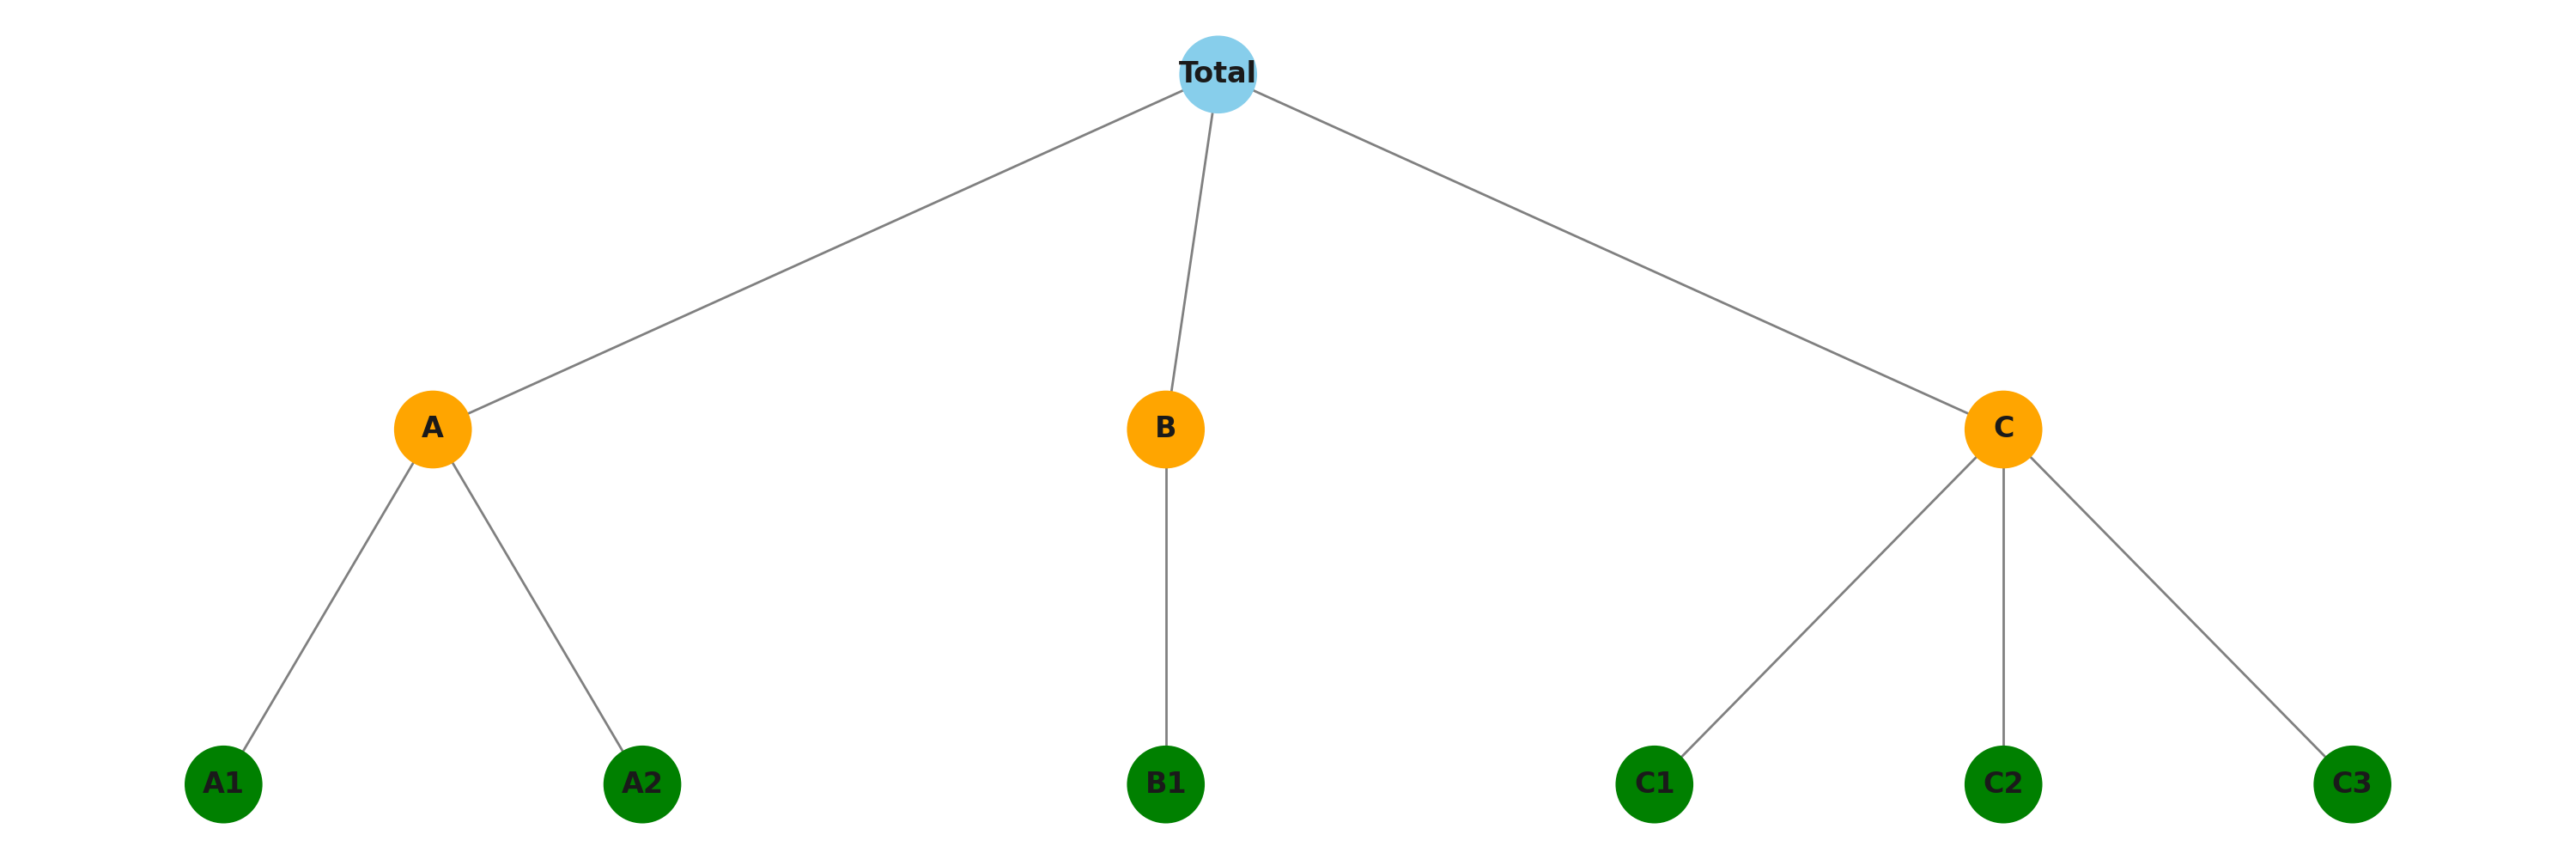
\includegraphics[width=\linewidth]{graph_nodes.png}
    \caption{Graph structure of hierarchical time series}
    \label{fig:hierarchy}
\end{figure}

\subsection{Matrix notation} \label{sec:matrix}

Consider a multivariate time series vector $ \mathbf{y}_t \in \mathbb{R}^n $ whose elements $y_{i,t}$,  $ i\in[0,n]$ are hierarchically linked. 
Assume the elements are ordered by traversal of the tree graph going from left to right at each level, top to bottom. 

We can thus distinguish the aggregated time series from the bottom-level signal $\mathbf{y}_t = [\mathbf{y}^{\mathrm{agg}}_t,\mathbf{b}_t]^{\top} $ with $\mathbf{y}^{\mathrm{agg}}_t \in \mathbb{R}^{n-m}$ and $\mathbf{b}_t \in \mathbb{R}^{m}$ with $m < n$ the number of bottom-level time series.
Each hierarchy can be defined by a summation matrix $\mathbf{S} \in \{0,1\}^{n,m}$ which maps the bottom-level time series to all signals in the hierarchy according to the aggregation constraints :

\begin{equation}
    \mathbf{y}_t = \mathbf{Sb}_t  \Leftrightarrow   \mathbf{y}_t = \begin{bmatrix}
 A_{n-m,m} \\
 I_{m}
\end{bmatrix}\mathbf{b}_t
    \label{eq:1}
\end{equation}

Where $I_m$ is the $m \times m$ identity matrix and $A_{n-m,m}$ dictates the time series aggregation.

In the example given in figure \ref{fig:hierarchy} :

\begin{equation}
    \begin{bmatrix}
    y_{t} \\
    y_{A,t} \\
    y_{B,t} \\
    y_{C,t} \\
    y_{A1,t} \\
    y_{A2,t} \\
    y_{B1,t} \\
    y_{C1,t} \\
    y_{C2,t} \\
    y_{C3,t}
  \end{bmatrix}=
  \begin{bmatrix}
    1 & 1 & 1 & 1 & 1 & 1\\
    1 & 1 & 0 & 0 & 0 & 0\\
    0 & 0 & 1 & 0 & 0 & 0\\
    0 & 0 & 0 & 1 & 1 & 1\\
    \hline \\
    \\
    & &  I_6& & \\
    \\
    \\
  \end{bmatrix}
  \begin{bmatrix}
    y_{A1,t} \\
    y_{A2,t} \\
    y_{B1,t} \\
    y_{C1,t} \\
    y_{C2,t} \\
    y_{C3,t}
  \end{bmatrix}
\end{equation}

In this framework, we define coherent forecasts as forecasts for which equation (\ref{eq:1}) holds. 
Traditionally, base (non-coherent) forecasts are noted $\hat{\mathbf{y}}_t$ and reconciled (coherent) forecasts $\tilde{\mathbf{y}}_t$.

\subsection{Point forecast Reconciliation} \label{point_rec}

Forecast reconciliation aims to make forecasts coherent with regards to the aggregation constraints of the hierarchy. 
To that end, typical reconciliation consists in mapping the base forecasts to forecasts of the bottom level time series $\hat{\mathbf{b}}_t = \mathbf{G}\hat{\mathbf{y}}_t$, which can then be aggregated using the summing matrix $\mathbf{S}$. 
Reconciled forecasts for all time series in the hierarchy can thus be recovered: 

\begin{equation}
\tilde{\mathbf{y}}_t = \mathbf{S}\hat{\mathbf{b}}_t = \mathbf{SG}\hat{\mathbf{y}}_t
\label{eq:recon}
\end{equation}

The matrix $\mathbf{G} \in \mathbb{R}^{m,n}$ in (\ref{eq:recon}) determines the reconciliation method. 

The simplest method is bottom-up, given by the matrix :  \[ \mathbf{G}~=~[\mathbf{0}_{m,n-m}|\mathbf{I}_{m,m}]. \]

In this approach only the bottom-level forecasts are considered and summed to recover aggregated signals. 
This method is optimal in that it recovers all information on the hierarchy using the minimal number of time series. 
However, in practice it can lead to excessive error as the most disaggregated time series often are the hardest to forecast due to low signal-to-noise ratio, high sparseness, or non-normality. 

In contrast, the top-down approach only uses the top-level time series' forecast, corresponding to : \[\mathbf{G} = [\mathbf{p}_{m,1}|\mathbf{0}_{m,n-1}] \] with $\mathbf{p}_{m,1}\in \left\{ 0,1\right\}^m$ the disaggregation proportions.
This approach inversely benefits from the most aggregated time series often being the most predictable, and thus having the most reliable forecast. 
In practice, the computation of relevant proportion might pose a problem, and using only an aggregated time series smooths out a large portion of information contained at lower levels of aggregation. 

The middle-out approach was thus proposed in \cite{bookhyndman} as a combination of both previous methods seeking to mitigate each of their problems.
The time series of an intermediate level are forecast, and the aggregation is done in a bottom-up manner for time series of higher levels and in a top-down manner for lower time series. 

An optimal reconciliation under the assumption of unbiased base forecasts was proposed under the name minimum trace \cite{MinT}. 
This method finds the matrix $\mathbf{G}$ which minimizes the trace of the covariance matrix $\mathbf{\Sigma}_t = Var[(\mathbf{y}_t - \tilde{\mathbf{y}_t})]$, whose diagonal terms are the error terms of the reconciled forecasts. 
Under the constraint $\mathbf{SGS} = \mathbf{S}$, which ensures reconciled forecasts remain unbiased, one can show :
\begin{equation}
\mathbf{G}=(\mathbf{S}^{\top} \mathbf{\Sigma}_h^{-1}\mathbf{S})^{-1}\mathbf{S}^{\top}\mathbf{\Sigma}_h^{-1}
\label{mint}
\end{equation}

Note that solving eq. \ref{mint} requires additional assumptions in order to estimate $\mathbf{\Sigma}$. 
For example $\mathbf{\Sigma} = k\mathbf{I}$ yields the ordinary least square (OLS) estimator.

The Game Theoretically OPtimal (GTOP) reconciliation was proposed in \cite{gtop} as a counterpoint to the minimum trace approach which relaxes the assumption of unbiasedness of base forecasts and does not require covariance matrix estimation.

The GTOP method interprets forecast reconciliation as a two-player zero sum game.
The forecaster selects a reconciliation operator, whereas an adversary chooses the realized bottom-level vector $y_t$ so as to maximize the forecaster's loss. 
The forecaster therefore solves a minimax problem that minimises the worst case change in loss induced by reconciliation. 
Thanks to the Pythagorean identity, Theorem~2 of \cite{gtop} shows that such a reconciled forecast is guaranteed to result in an improvement on the loss, with equality if the base forecasts are coherent.

One can show that when the loss is the squared error, this method reduces to an L2-projection on the subspace of coherent forecasts $\mathcal{A} = \left\{\mathbf{y} \in \mathbb{R}^n | \mathbf{y}=\mathbf{S}\mathbf{y}_{[n-m,m]}\right\}$.

\begin{equation}
   \tilde{\mathbf{y}}_{\mathrm{gtop}} = \underset{\tilde{\mathbf{y}}\in \mathcal{A}}{\mathrm{arg}\mathrm{min}} \|\mathbf{A\hat{y}-A\tilde{y}}\|^2
\end{equation}

Where $\mathbf{A} = \mathrm{diag}(\sqrt{a_i})$ accounts for each time series' weighing factor.

% \begin{equation}
% \|\mathbf{y}-\tilde{\mathbf{y}}_{\mathrm{gtop}}\|^2 \leq \|\mathbf{y}-\hat{\mathbf{y}}\|^2,  \forall \mathbf{y} \in \mathcal{A}
% \end{equation}

\subsection{Probabilistic forecast reconciliation}\label{prob_rec}

In order to implement probabilistic reconciliation, one must first define the notion of coherence for probabilistic forecasts. 
Given the probability triple $(\mathbb{R}^m, \mathcal{F}_m, \mathbb{P}_m)$ with $\mathcal{F}_m$ the Borel $\sigma$-algebra on the sample space $\mathbb{R}^m$, and $\mathbb{P}_m$ a forecast probability on the $m$ bottom level time series. 
The summing matrix $\mathbf{S}$ defines a linear mapping $\mathbf{s}(\cdot) : \mathbb{R}^m  \mapsto \mathbb{R}^n$ according to the hierarchical aggregation.
A coherent forecast space $(\mathbb{R}^n, \mathcal{F}_n,\mathbb{P}_n)$ satisfies :

\begin{equation}
    \mathbb{P}_n(\mathbf{s}(\mathcal{B})) = \mathbb{P}_m(\mathcal{B}) \;\;\;\; \forall \mathcal{B}\in \mathcal{F}_m
\end{equation}

Let $(\mathbb{R}^n, \mathcal{F}_n,\hat{\mathbb{P}}_n)$, an incoherent forecast space and $\mathbf{g}(\cdot) : \mathbb{R}^n  \mapsto \mathbb{R}^m $ a linear mapping, the reconciled probability measure $\tilde{\mathbb{P}}_n$ of $\hat{\mathbb{P}}_n$ with respect to the mapping $\mathbf{g}(\cdot)$ is such that:

\begin{equation}
   \tilde{\mathbb{P}}_n(\mathbf{s} (\mathcal{B})) = \mathbb{P}_m(\mathcal{B}) = \hat{\mathbb{P}}_n(\mathbf{g}^{-1}\left ( \mathcal{B}\right )) \;\; \forall \mathcal{B}\in \mathcal{F}_m
\end{equation}

Where $ \mathbf{g}^{-1} (\mathcal{B}) = \{ \mathbf{y} \in \mathbb{R}_n \; | \; g(\mathbf{y}) \in \mathcal{B} \} $ is the pre-image of $\mathcal{B}$ in $\mathcal{F}_n$. 
This definition extends the concept of forecast reconciliation in a probabilistic setting. 
In practice, the first and easiest approach to reconciliation is to assume that forecasts follow the same parametric distribution at all levels. 
For example, assuming independent Gaussian distributions at the bottom levels, the aggregated distribution can be easily recovered using the well-known closed-form result for sums of Gaussian-distributed random variables. 

However, having to assume a specific parametric form for the forecast distribution is too restrictive to be useful in most practical situations \cite{ANR_book}.
A simple framework is thus introduced by \cite{probreconciliation}  for nonparametric probabilistic reconciliation based on bootstrapped future paths. 
Each bootstrapped sample can be reconciled using the same methods as previously introduced for point forecasts, in order to recover a reconciled distribution.
In this situation, optimal reconciliation can be obtained by minimizing a multivariate proper scoring rule:

\begin{equation}
    \underset{\mathbf{G}}{\mathrm{argmin}} \; \mathbb{E}\left[ \mathcal{S}(\mathbf{SG}\hat{\mathbf{y}}^i_t, \mathbf{y}_t) \right]
\end{equation}

where $i\in\{0, N_b\}$ denote bootstrap samples, $\mathbb{E}$ the bootstrap average and $\mathcal{S}$ is a proper scoring rule. 

Another method, proposed by \cite{PERMBU}, seeks to implement a probabilistic bottom-up approach. 
Applying regular bottom-up for probabilistic forecasts would require modeling the joint distribution of all bottom-level forecasts, which is impractical.
The PERMBU method thus proposes to use a copula \cite{Copula_book} approach to model the joint distribution of the empirical forecast marginals. 
Thus, the method obtains a coherent probabilistic forecast by ordering samples from the marginal distributions according to empirical copulae computed from forecast errors. 
To further enhance efficiency, the potentially high-dimensional copula is decomposed into lower-dimension copulae by grouping together the children of each aggregated series. 

\subsection{End-to-end coherent probabilistic forecasting}

Recent advances in hierarchical time series forecasting have shifted focus towards end-to-end probabilistic models that directly generate coherent predictive distributions, eliminating the need for post-hoc reconciliation. 
These state-of-the-art approaches integrate the requirements of hierarchy coherence into deep learning architectures, allowing the forecasting model to natively produce forecasts that respect aggregation constraints across all levels of the hierarchy.

In general, two strategies can be identified to enforce probabilistic coherence during neural network training: 



\begin{itemize}
    \item \textbf{Coherence as Regularization.}
In this approach, coherence is encouraged by augmenting the loss function with a regularization term that penalizes the incoherence of forecasts. 
Architectures such as SHARQ \cite{SHARQ} and PROFHIT \cite{PROFHIT} exemplify this method. 
They compute the degree of incoherence—typically measured as the norm of the difference between base and reconciled predictions—and incorporate it as an additional penalty within the training objective. 
This formulation enables standard training pipelines and permits a trade-off between predictive accuracy (negative log-likelihood, CRPS...) and hierarchical coherence via tunable hyperparameters. 
A key advantage of this approach is its ability to model weakly hierarchical time series---time series which do not strictily adhere to their aggregation constraints. 

\item \textbf{Coherence as a Differentiable Constraint.}
Alternatively, coherence can be embedded as a hard or soft constraint directly on the output forecasts, enforced by differentiable operations within the model. 
This strategy is adopted in architectures such as HierE2E \cite{HierE2E} and CLOVER \cite{CLOVER}, where the forecast outputs are projected onto the space of coherent predictions. 
Typically, this is conducted using a reconciliation layer which samples from the predictive distribution and projects the forecast future paths onto the coherent subspace using any point reconciliation method. 
Once sufficient statistical information is recovered the model produces a probabilistic output which is coherent by construction at every level.

\end{itemize}

Both strategies have their advantages and drawbacks. 
While the regularization approach affords flexibility across both distribution choice and reconciliation method at the cost of potentially imperfect coherence, the constraint-based view enables strict coherence and eliminates a performance-coherence trade-off at the cost of the necessity of sampling from the predictive distribution.

These end-to-end frameworks make significant progress in scalable and accurate probabilistic forecasting for hierarchical settings, it is however important to note that they have thus far only been evaluated on standard benchmark datasets such as those from the M competitions or retail sales data.
These datasets do not necessarily reflect the full complexity and unique challenges characteristic of private debt markets, such as data sparsity, non-Gaussian and heavy-tailed distributions or lack of clear seasonality. 
As a result, the effectiveness and robustness of these state-of-the-art methods in the context of private debt forecasting remain largely unexplored.

Given the growing literature on end-to-end probabilistic hierarchical time series forecasting, we focus our attention on the three most promising and representative architectures: PROFHIT, HierE2E, and CLOVER. 
These models cover both distinct approaches for ensuring forecast coherence, and ensure robustness and scalability through the use of probabilistic multivariate forecasters.
All use methods which can train end-to-end on the whole hierarchy at once - in contrast to models using first point then quantile reconciliation like SHARQ or DYCHEM \cite{SHARQ}, \cite{DYCHEM} or models using a top-down approach \cite{Dirichlet}.

\textit{\textbf{PROFHIT}} is an end-to-end architecture designed to produce coherent probabilistic forecasts over a hierarchy of time series. 
The method leverages neural networks to jointly learn the temporal patterns and the hierarchical dependencies between time series, with an explicit integration of probabilistic coherence as part of the training process.

At a high level, PROFHIT proceeds in two main stages: base probabilistic forecasting and hierarchical refinement.

\begin{itemize}

    \item \textit{Base Forecast Model}: Input time series spanning all levels of the hierarchy are simultaneously ingested by a multivariate neural forecasting model. 
    This model generates, for each time series $y_i$, a set of distributional parameters, specifically the mean $ \mu_i $ and standard deviation $ \sigma_i $, thereby parameterizing a univariate Gaussian predictive distribution $\mathcal{N}(\mu_i, \sigma_i^2)$ for each series.

    \item \textit{Refinement Module}: To explicitly account for dependencies between the forecast distributions across the hierarchy, PROFHIT introduces a refinement module. 
    Here, the initial base forecast parameters $(\mu_i, \sigma_i)$ from all series are fed into a set of dense, feed-forward layers that produce refined distributional parameters $( \hat{\mu}_i, \hat{\sigma}_i )$.

    \item \textit{Coherence Enforcement via Soft Regularization}: PROFHIT ensures forecast reconciliation through its training objective, which not only maximizes the series-wise likelihood but also regularizes for hierarchical coherence. 
    Instead of treating coherence as a hard constraint, PROFHIT introduces a “soft” distributional consistency regularization term. 
    Coherence is quantified using a symmetrized variant of the Kullback-Leibler (KL) divergence between the forecast distributions of parent nodes and the sum of their children. 
    Under the assumption of independent univariate Gaussians, one can express simply the distribution of the sum of children nodes as :
    
    \begin{equation}
     \mathbb{P}(\underset{j\in \mathcal{C}_i}{\sum}y_{j,t}| \mu_j , \sigma_j) =  \mathcal{N}(\underset{j\in \mathcal{C}_i}{\sum}\mu_j, { \underset{j\in \mathcal{C}_i}{\sum}\sigma^2_j})
    \end{equation}

    Using the known result on the closed form of the Kullback-Leibler divergence of univariate Gaussians, the inconsistency loss can be expressed as such :

  
    \begin{multline} 
    \mathrm{KL}(\mathbb{P}(y_i),\mathbb{P}(\underset{j\in \mathcal{C}_i} {\sum}y_{j,t})) + \mathrm{KL}(\mathbb{P}(\underset{j\in \mathcal{C}_i} {\sum}y_{j,t}),\mathbb{P}(y_i))+ 1 = \\ \cfrac{\sigma_i^2 + \left(\mu_i - \underset{j\in \mathcal{C}_i}{\sum}\mu_j \right)^2}{2{\underset{j\in \mathcal{C}_i}{\sum}\sigma^2_j}} + \cfrac{\underset{j\in \mathcal{C}_i}{\sum}\sigma^2_j + \left(\mu_i - \underset{j\in \mathcal{C}_i}{\sum}\mu_j \right)^2 }{2\sigma_i^2}
    \end{multline}

\end{itemize}

In summary, PROFHIT achieves end-to-end probabilistic coherence by combining a multivariate neural forecasting model with a refinement module that explicitly models distributional dependencies across all time series in the hierarchy.
At the cost of strong distributional assumptions (independently distributed Gaussian random variables), PROFHIT efficiently penalizes incoherence at the distributional level without the need for computationally expensive sampling. 
This approach ensures that the learning process encourages both accurate and hierarchy-consistent probabilistic forecasts.

\textit{\textbf{HierE2E}} introduces probabilistic forecast coherence directly within the neural network training loop by integrating a reconciliation step into the forward pass of a deep probabilistic time series model. 
This approach offers a principled solution for producing forecasts that are not only distributionally calibrated but also satisfy hierarchical aggregation constraints by construction.

\begin{itemize}
     
\item \textit{Base Forecast Model}: HierE2E is built atop DeepAR \cite{DeepAR}, a widely used multivariate probabilistic forecasting framework that models each time series with an auto-regressive recurrent neural network (RNN). 
DeepAR generates the parameters of the predictive distribution---such as the mean $ \mu_i $ and standard deviation $\sigma_i $ in the case of Gaussian marginals---conditioned on the RNN’s hidden state.

\item \textit{Differentiable Sampling}:
In order to achieve probabilistic coherence, HierE2E introduces reconciliation within the stochastic forecast generation path. 
During both training and inference, samples are drawn from the marginal distributions at all levels of the hierarchy in a differentiable manner using a reparameterization trick. 
This technique allows the stochasticity of the sampling process to remain trackable for backpropagation, facilitating gradient-based learning even through the sampling step.

\item \textit{Hierarchical reconciliation}: These marginal samples are subsequently reconciled to enforce the aggregation constraints inherent in hierarchical structures. 
Specifically, the reconciliation is performed using a projection method which is a simplified version of the GTOP technique used in point forecasting \cite{gtop}. 
Under these simple assumptions, a time invariant projection matrix can be computed, making the reconciliation process efficient and differentiable. 
By characterizing the coherent subspace as the nullspace of a matrix $A = \left[ I | - S  \right]$ where $S$ is the aggregation matrix, one can obtain the projection matrix : 

\begin{equation}
    M = I - A^{\top}(AA^{\top})^{-1}A. 
\end{equation}

Such that $\tilde{\mathbf{y}}_t = M\hat{\mathbf{y}}_t$ satisfies :

\begin{multline}
    \tilde{\mathbf{y}}_t = \underset{\mathbf{y}\in \mathbb{R^n}}{\mathrm{argmin}} \|\mathbf{y} - \hat{\mathbf{y}}_t  \|^2 \\
    \mathrm{s.t.} \; A\mathbf{y} = 0
\end{multline}

\item \textit{Loss computation}: Once sufficient projected samples are obtained, their empirical distributions are used to recover the necessary summary statistics for loss computation. 
For example, the mean and variance of the reconciled samples can be used to calculate the negative log-likelihood loss under a Gaussian assumption; alternatively, a collection of quantiles can be computed to facilitate the use of quantile-based scoring rules such as the Continuous Ranked Probability Score (CRPS).

\end{itemize}

In summary, HierE2E tightly couples modern deep probabilistic forecasting (via DeepAR) with hierarchical reconciliation, offering a fully end-to-end trainable pipeline for coherent probabilistic forecasts. 
Modeling all time series as univariate marginals, HierE2E generates reconciled future paths, sampling from all time series in the hierarchy, and projecting on the coherent subspace, in a differentiable manner. 


\textit{\textbf{CLOVER}} advances hierarchy-aware probabilistic forecasting by explicitly modeling the dependencies among the bottom-level time series, thereby lifting the independence assumption inherent in earlier frameworks such as HierE2E and PROFHIT. 
The core innovation of CLOVER lies in the use of a Gaussian factor model to capture a structured, low-rank covariance matrix across all bottom-level series.

\begin{itemize}
     
\item \textit{Forecast Model}: CLOVER augments the MQCNN (Multi-Quantile Convolutional Neural Network) \cite{MQCNN} architecture with a cross-series multi-layer perceptron (MLP) layer. 
This dense layer enables information sharing across all time series during representation learning, ensuring the bottom-level forecasts reflect both individual series characteristics and their interactions within the hierarchy.


\item \textit{Gaussian factor model}: Instead of producing only independent marginal distributions for each bottom time series, the augmented MQCNN forecasts the parameters of a Gaussian factor model: Mean $\mu_i$ and standard deviation $\sigma_i$ for each bottom-level series as well as factor loading vectors $\mathbf{F}_i$, which collectively specify a low-rank, non-diagonal covariance structure across all bottom-level series. 
This parameterization yields a multivariate Gaussian distribution for the bottom-level forecasts, with a structured covariance matrix that efficiently encodes both variance and dependency through latent factors.

\begin{multline}
    \mathrm{Cov}(\hat{y}_{i,t}, \hat{y}_{j,t}) = \sigma^2_i\delta_{ij} + \mathbf{F}_{ik} \mathbf{F}_{j}^k \\ 
    \forall (i,j) \in  \llbracket 0, m \rrbracket 
\end{multline}


\item \textit{Differentiable Sampling and Reconciliation}:
The structured multivariate Gaussian produced by CLOVER lends itself to differentiable sampling, accomplished using the following reparameterization trick: 

\begin{multline}
    \hat{\mathbf{y}}_t = \hat{\mathbf{\mu}}_t + \mathbf{\hat{\sigma}}_t \mathbf{z}_t + \hat{\mathbf{F}}^k\mathbf{\varepsilon}_{k,t}\\
    \mathbf{z}_t \sim \mathcal{N}(0,\mathbf{I}_n) \,\varepsilon_{k,t} \sim \mathcal{N}(0,\mathbf{I}_k)
\end{multline}

This enables the network to generate coherent, correlated samples across all bottom-level series while retaining full differentiability for training with backpropagation. 
In order to extend coherent forecasts to the entire hierarchy, the sampled bottom-level forecasts are reconciled upwards using the bottom-up reconciliation approach. 
Through this summing procedure, coherent forecasts are computed for all aggregate nodes in the hierarchy.

\item \textit{Loss Computation and Training Objectives}: CLOVER’s flexible probabilistic modeling supports a variety of training objectives. 
Similarly to HierE2E, proper scoring rules such as the negative log-likelihood or CRPS (Continuous Ranked Probability Score) can be applied to the reconciled outputs. 
Furthermore, CLOVER supports multivariate scoring rules, such as the energy score, to evaluate and optimize the joint distributional accuracy of the bottom-level forecasts.
\end{itemize}

In summary, CLOVER models multivariate dependencies among bottom-level time series via a low-rank Gaussian factor model. 
By capturing cross-series correlations directly in the covariance structure and integrating this with end-to-end differentiable sampling and bottom-up reconciliation, CLOVER enables the production of distributionally coherent, probabilistically calibrated forecasts throughout the entire hierarchy. 
This approach overcomes the independence limitations of prior methods and provides a scalable solution for complex domains where accurate modeling of inter-series dependence is critical. 
However, this method is limited to bottom-up aggregation due to the complexity of modeling multivariate dependencies across all the hierarchy. 

\section{Methodology}
\subsection{Data collection}

The primary dataset utilized in this study consists of Italian private debt data, retrieved from the official statistical database of the Bank of Italy, specifically the \textit{Financing and Funding by Sector and Geographical Area} statistical bulletin. 
This data source provides comprehensive coverage of private debt aggregates, enabling a granular analysis of credit dynamics across distinct economic and geographical partitions.

The main variable of interest is the aggregate of loans, following the definition provided by Banca d'Italia: 
\say{The aggregate includes the following technical forms: current accounts, mortgages, credit cards, salary-backed loans, personal loans, financial leasing, factoring transactions, other financing (e.g. commercial paper, pawned loans, annuity discounts), reverse repurchase agreements, bad debts (including bad debts on expired securities), and some residual components. Assets sold and not written off are included.} 
In addition to total loans, we consider sub-aggregates such as bad loans within this aggregate (see Figure \ref{fig:maps}).

\begin{figure*}
    \centering
     \begin{subfigure}[b]{0.47\textwidth}
         \centering
         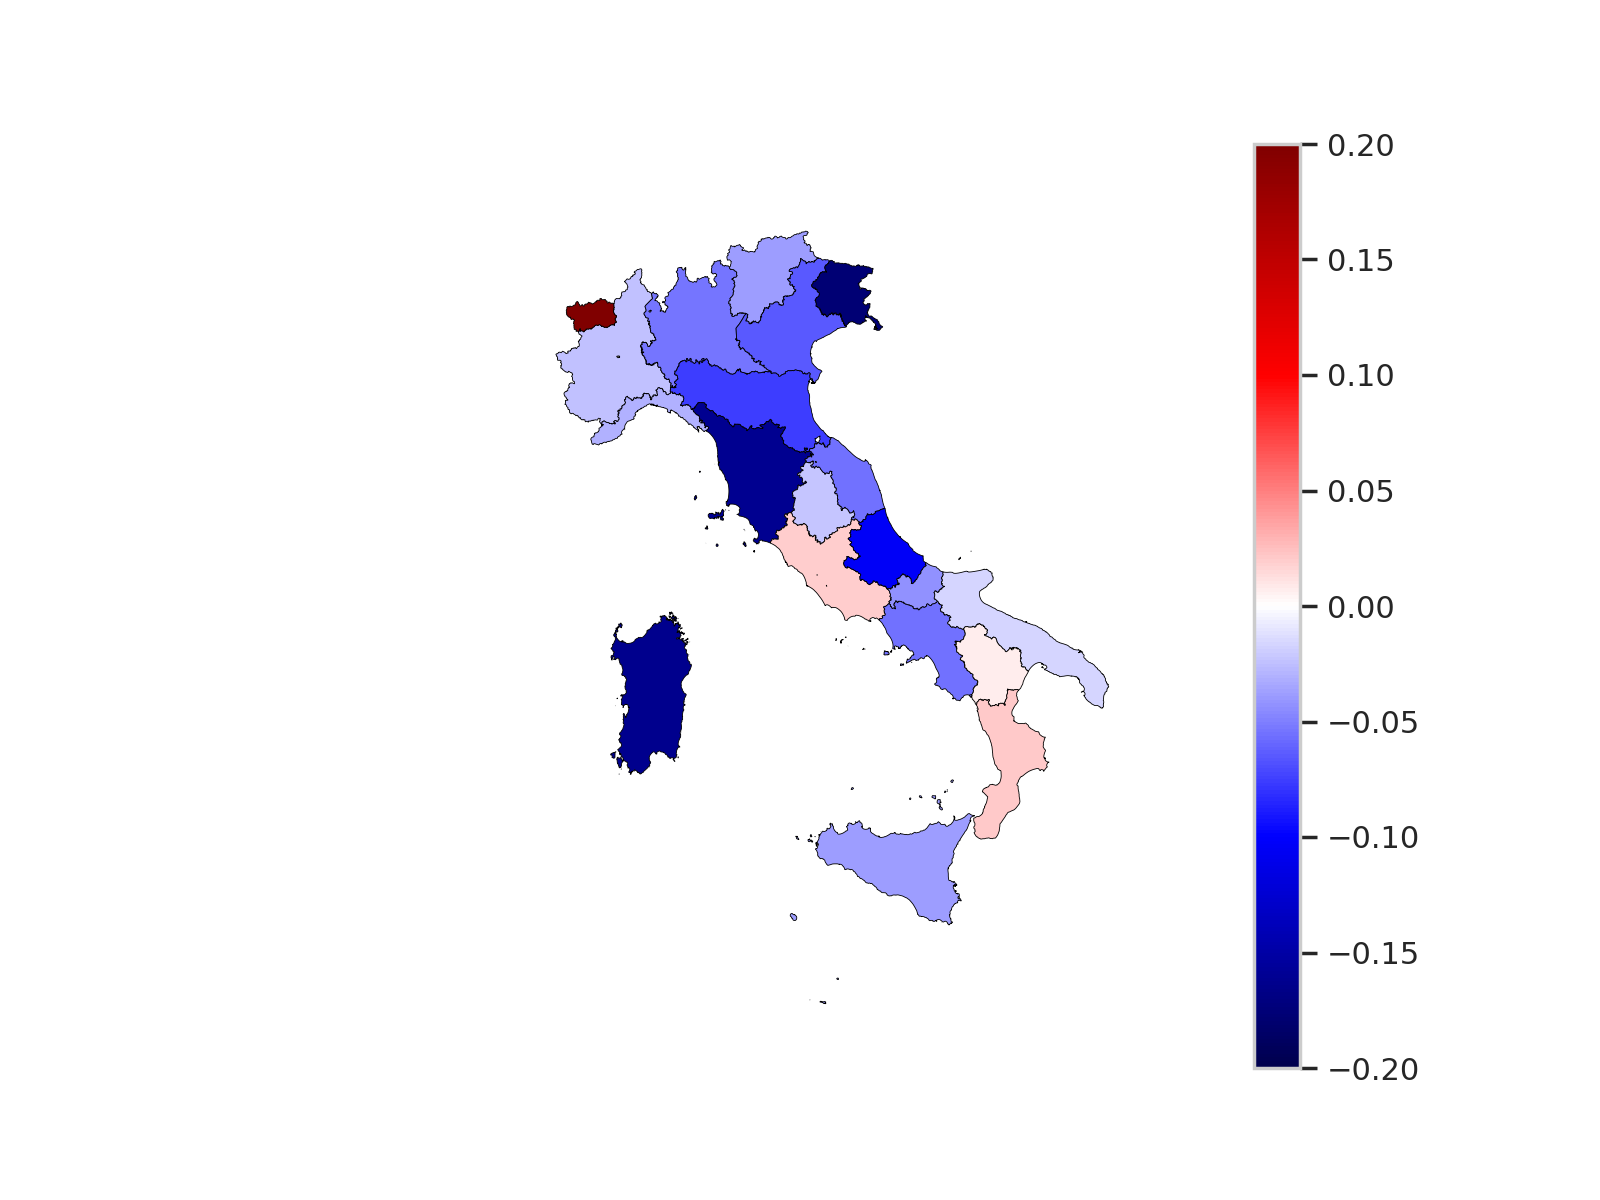
\includegraphics[width=\textwidth]{bad_loans_map.png}
         \caption{12 months percent change in originations (28-02-2025)}
         \label{fig:sub1}
     \end{subfigure}
     \hfill
     \begin{subfigure}[b]{0.47\textwidth}
         \centering
         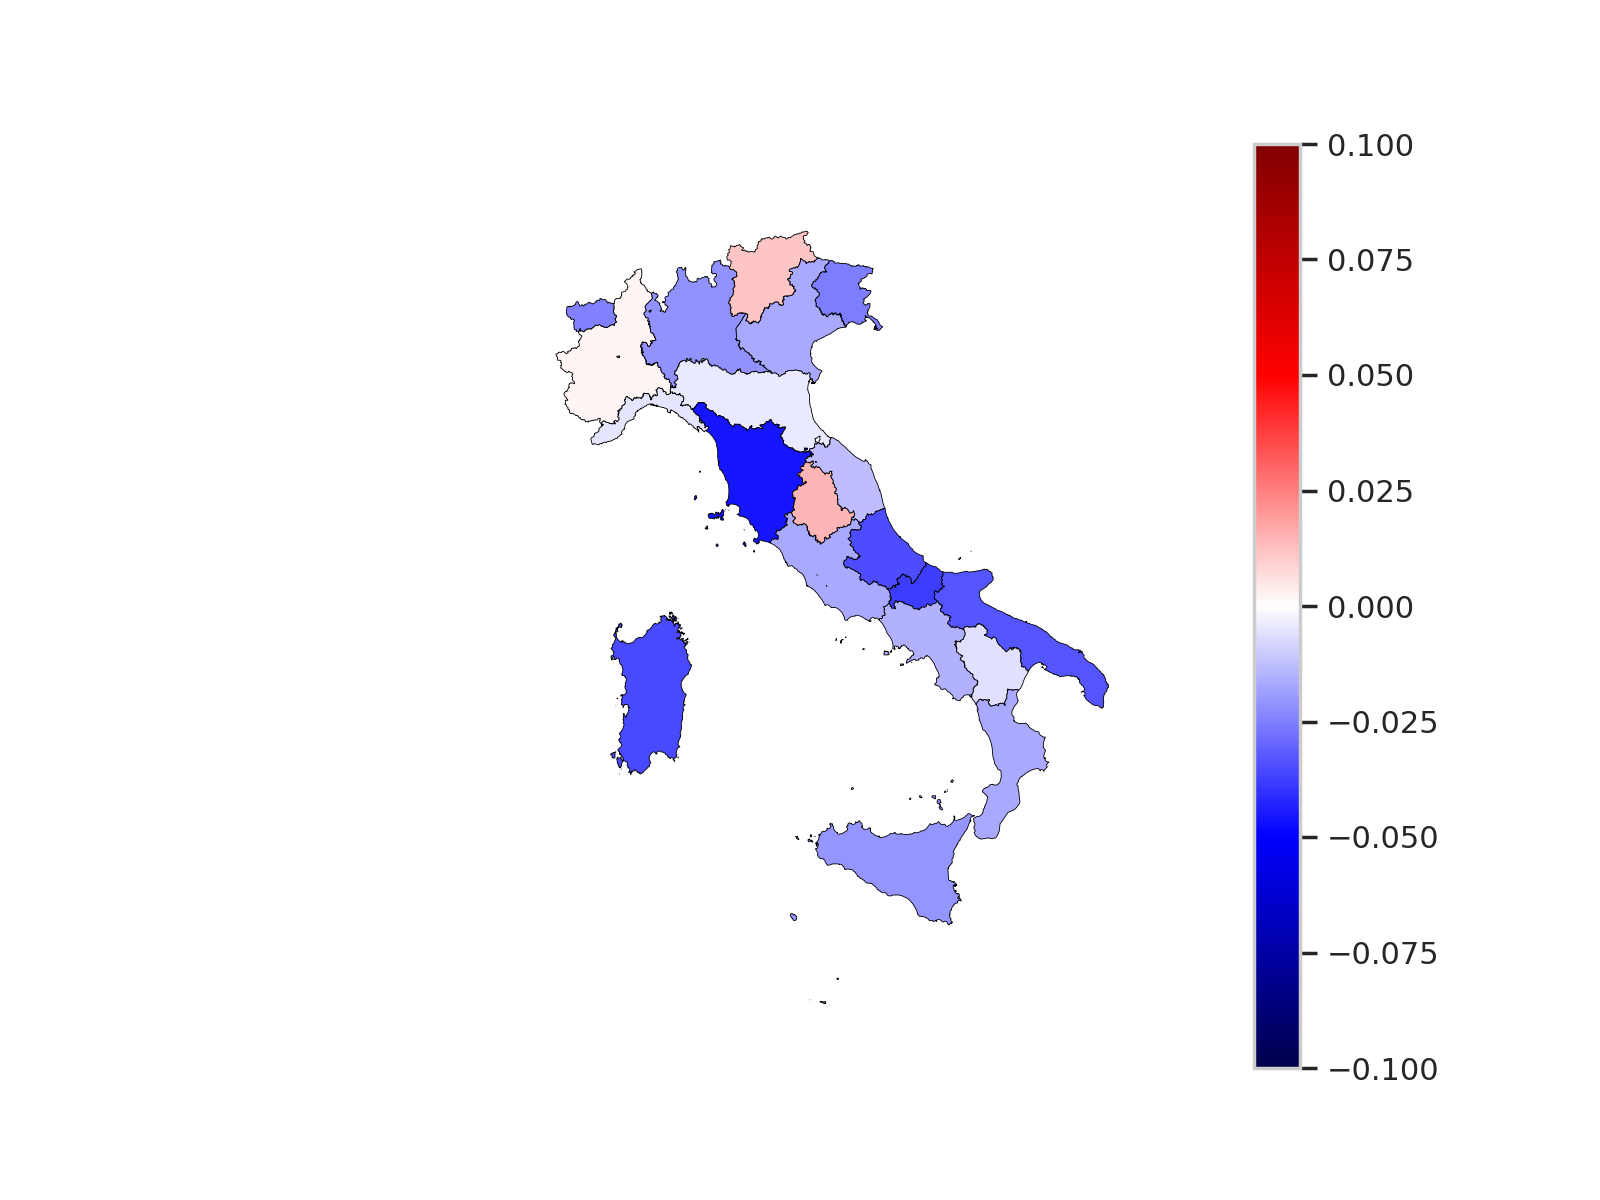
\includegraphics[width=\textwidth]{orig_loans_map.png}
         \caption{12 months percent change in bad debt (28-02-2025)}
         \label{fig:sub2}
     \end{subfigure}
     \hfill
        \caption{Maps of italian regions showing the hierarchical loan aggregate data from the central bank of italy.}
        \label{fig:maps}
\end{figure*}


The data is disaggregated along two main dimensions: geography and sector. 
Geographical disaggregation is available down to the province level, while sectoral information follows the ESA 2010 classification \cite{esa2010}, available down to subsectors. 
For the purposes of hierarchical modeling and to mitigate sparsity and data quality issues, we truncate both geographical and sectoral hierarchies. 
Specifically, we exclude the provincial-level granularity, as reporting is often inconsistent and signals are predominantly sparse and incomplete at this level.

The final hierarchical structure employed in this study thus comprises 126 time series, encompassing 1 national total, 5 macro-regions (as per the nomenclature adopted by the Bank of Italy), 20 regions, each further divided into 5 sectors. 
This configuration provides a balance between granularity and data availability, ensuring each node of the hierarchy contains sufficiently informative signals while maintaining computational tractability. 
The dataset spans approximately 165 monthly observations, covering the period from June 2011 to the most recent available data, which presents a data sufficiency challenge for data-hungry neural network models as the hierarchical disaggregation increases the number of time series.

Using the truncated hierarchy, we find no missing values in the dataset. 
However, some small residuals are observed when aggregating values up the hierarchy. 
These discrepancies are minimal and attributable to floating point approximations inherent to digital computation. 
To eliminate potential confusion for the modeling process and to strictly enforce the aggregation constraints, we reconstruct the dataset by aggregating (summing) the bottom-level time series.
This procedure ensures that all higher-level nodes in the hierarchy are determined solely and consistently by their constituent series, thereby guaranteeing strict hierarchical consistency.

This study focuses on six-month ahead forecasts of the loan aggregates. 
To ensure robust performance evaluation and model generalization, we employ a conventional train-validation-test split. 
The two most recent years of data are reserved as the test set for out-of-sample evaluation. 
The year preceding the test period serves as the validation set, which is utilized during model training for early stopping and hyperparameter selection, effectively mitigating overfitting. 
The remaining historical data is used for model training.

Relevant context is incorporated through exogenous macroeconomic features. 
These monthly features are sourced from the Eurostat statistical database and include indicators such as gross domestic product (GDP), interest rates on government bonds, the harmonized consumer price index (HICP), and employment statistics. 
These covariates provide global exogenous information which informs the whole hierarchy and helps the model focus on internal dynamics and react accordingly to changes in the global economy. 
In addition, the models are provided with the future values of a temporal exogenous feature encoding the month of the year. 
This allows the models to explicitly capture seasonal patterns in the loan data. Furthermore, static exogenous features are constructed using one-hot encoding to describe each time series' position within the hierarchy. 
By encoding the hierarchical membership (i.e. macro-region, region, sector) for each node, the model is able to recognize structural relationships among series, such as which regions belong to the same macro-region, thus facilitating information sharing and improving the coherence of hierarchical predictions.

\subsection{Model Design}

\begin{figure*}
    \centering
     \begin{subfigure}[b]{\textwidth}
         \centering
         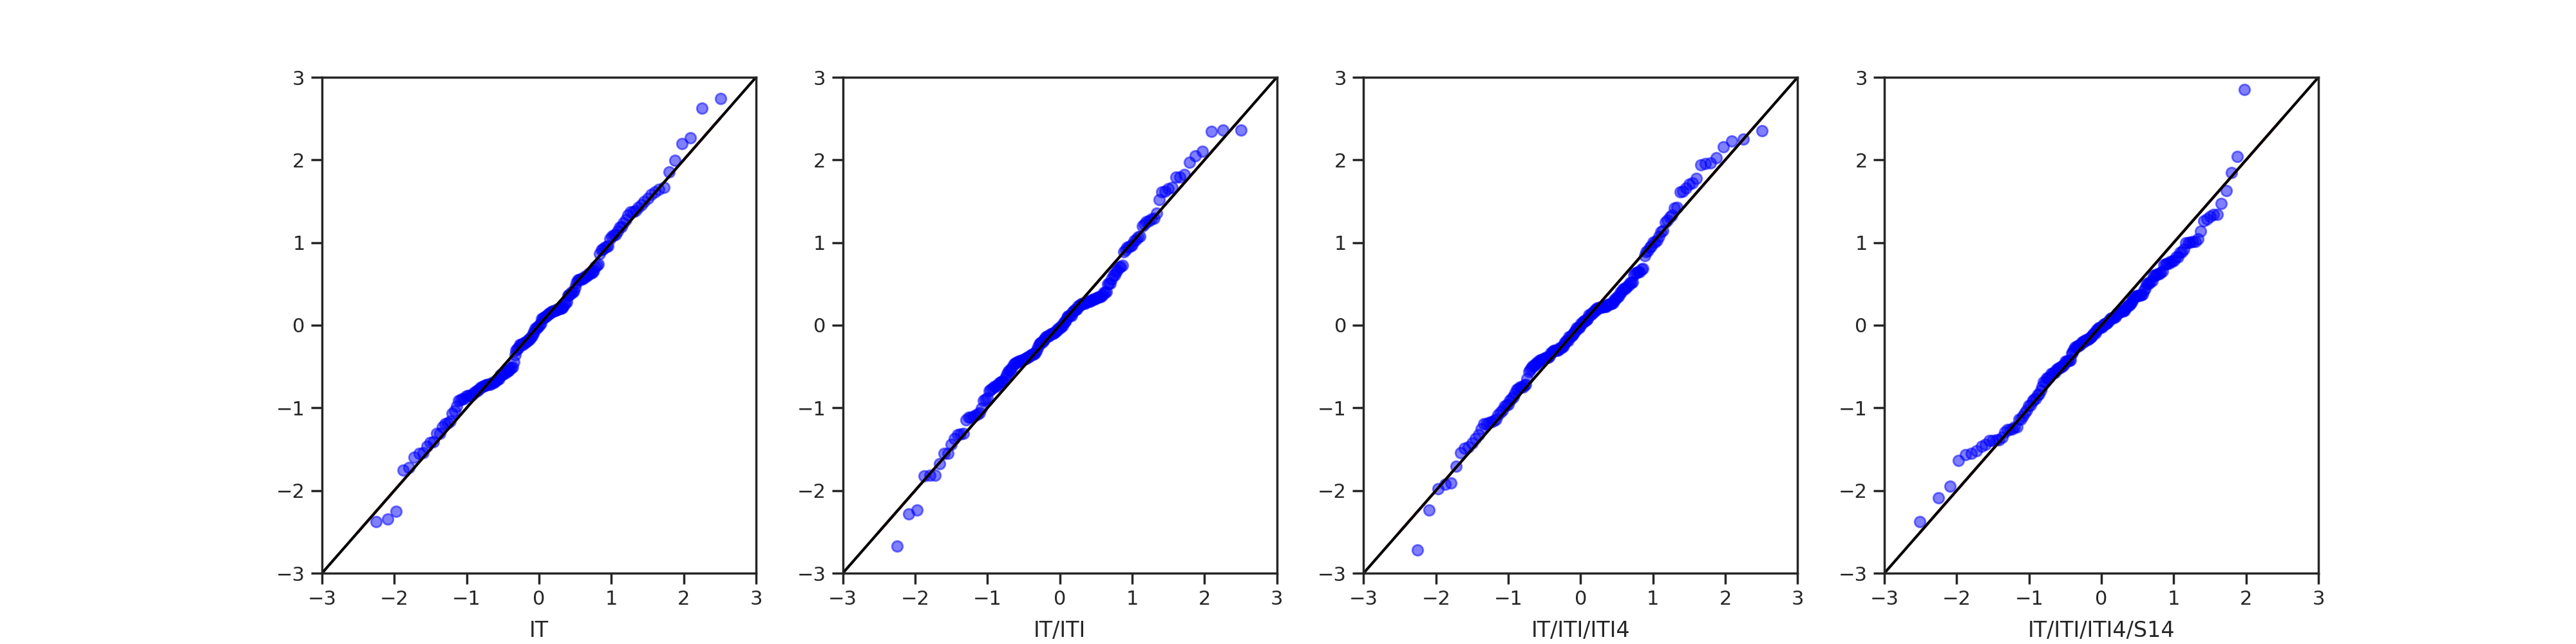
\includegraphics[width=\textwidth]{QQplots_lazio.png}
         \caption{Q-Q plots along the hierarchy: Italy $\rightarrow$ Central Italy $\rightarrow$ Lazio $\rightarrow$ Households in Lazio.}
         \label{fig:qqsub1}
     \end{subfigure}
     \begin{subfigure}[b]{\textwidth}
         \centering
         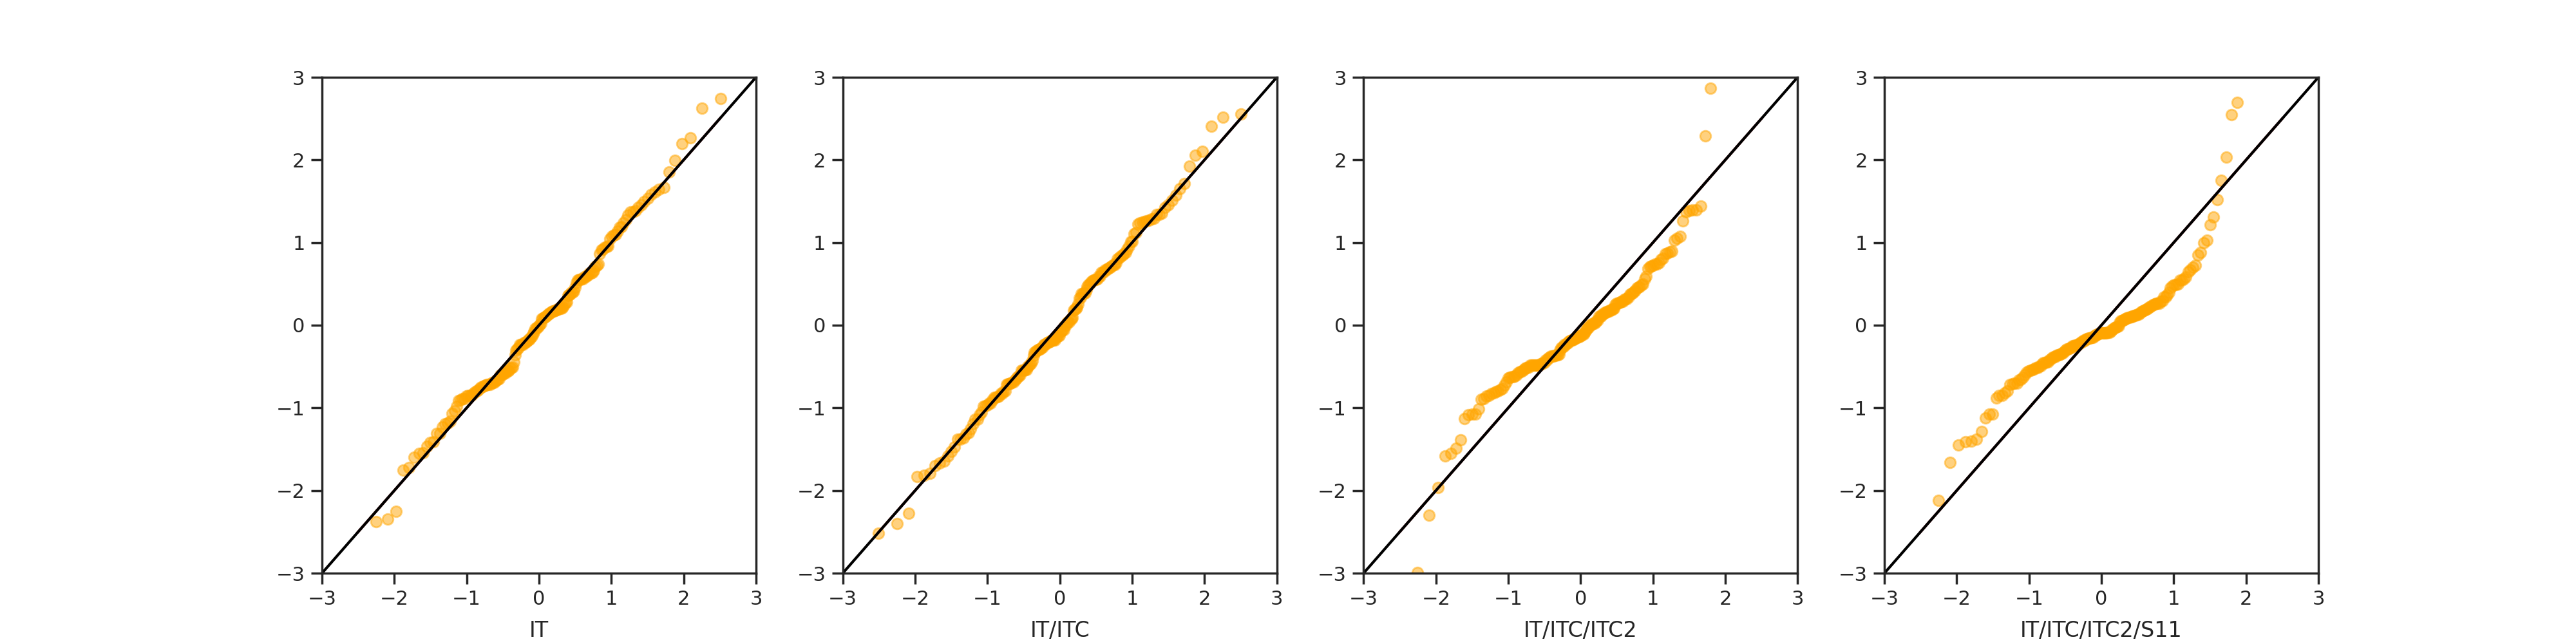
\includegraphics[width=\textwidth]{QQplots_valee.png}
         \caption{Q-Q plots along the hierarchy: Italy $\rightarrow$ Northwest Italy $\rightarrow$ Valle d'Aosta $\rightarrow$ Non-Financial Companies in Valle d'Aosta.}
         \label{fig:qqsub2}
     \end{subfigure}
     \hfill
        \caption{
Quantile-Quantile (Q-Q) plots of loan origination returns at each level of aggregation in the hierarchy. From left to right, each subplot represents a further step down the hierarchy. The first disaggregation path (a) traces from the national level (Italy) to Central Italy, then to the Lazio region, and finally to the Households sector within Lazio. The second path (b) displays the decomposition from Italy to Northwest Italy, then to the Valle d'Aosta region, and finally to Non-Financial Companies in Valle d'Aosta. The Q-Q plots reveal that the data along the first path exhibits an approximately Gaussian distribution at all levels. In contrast, the second path demonstrates heavier tails, especially at lower aggregation levels.
}
        \label{fig:qqplots}
\end{figure*}

In this study, we implement and compare three hierarchical probabilistic forecasting frameworks: PROFHIT, HierE2E, and CLOVER. 
For all models, predictive distributions are parameterized as Gaussian. 
Indeed, the Gaussian assumption is the basic distribution with which these frameworks have been used and benchmarked. 

Our choice of Gaussian predictive distributions across all models is further supported by empirical analysis of the marginal distributions of the time series in our dataset. 
As illustrated in Figure~\ref{fig:qqplots}, Q-Q plots at various levels of the hierarchy demonstrate that, in most cases, the distribution of loan origination returns is well-approximated by the Gaussian distribution—particularly at more aggregated levels. 
The appropriateness of the Gaussian assumption in our setting is attributable to the fact that we do not disaggregate to highly granular, elementary levels where the signal might be sparse or driven by count processes. 
For example, in datasets such as the M5 competition, which feature highly disaggregated retail sales at the store-item level, waiting time distributions or the Poisson distribution are more suitable at the bottom of the hierarchy due to the prevalence of discrete counts and zero inflation. 
In contrast, the credit dataset analyzed here retains sufficient aggregation at all levels, making the Gaussian assumption a reasonable and pragmatic modeling choice.  
We note, however, that in certain disaggregation paths—particularly at the lowest levels of the hierarchy—there is some visual evidence of heavier tails. 
A more detailed investigation into the sources and implications of these fatter tails is beyond the scope of the present study.

This choice enables the application of Reversible Instance Normalization (RevIN) \cite{revin}, a state-of-the-art approach for mitigating distribution shift and non-stationarity in time series forecasting.

RevIN operates by computing the mean and standard deviation of each input window and normalizing the inputs such that the model learns from stationary data. 
Inference entails re-scaling the predicted outputs to the original scale of the data, ensuring forecasts are expressed in the proper magnitude. 
Notably, RevIN itself acts as a global skip connection, allowing non-stationary statistical information to bypass the main model while the core network focuses on normalized signals.

To further hedge against potential distributional jumps between the input sequence and future values, 
the RevIN framework incorporates learnable parameters for both shift and scale during output re-scaling.

In this work, we extend RevIN to accommodate parameterized probabilistic outputs, specifically modeling predictive distributions as Gaussians. 
For each forecast, the normalized mean $\mu_{\text{norm}}$ and standard deviation $\sigma_{\text{norm}}$ are re-scaled. 
Additionally, for the CLOVER framework, the factor loading vectors are also scaled directly in order to recover the correct scaling in the covariance matrix by applying: 
\begin{align*}
    \mu_i &= \mu_{i}^\text{norm} \cdot \mu_i^\text{revin} + \sigma_i^\text{revin}  \,,\\
    \sigma_i &= \sigma_{i}^\text{norm} \cdot (\sigma_i^\text{revin}+ \epsilon) \,, \\
    \mathbf{F}_{i} &= \mathbf{F}^\text{norm}_i \cdot \frac{\sigma_i^\text{revin}}{\sqrt{r}}\,.
\end{align*}

where $\epsilon$ is a small positive constant ensuring numerical stability and $r$ is the size of the factor vector.

This unified approach enables each model not only to address non-stationarity in the target signals but also to maintain probabilistic calibration and coherent scale in both the mean and uncertainty forecasts.

We observe that the original forecasting neural networks proposed in these frameworks (PROFHIT, HierE2E, and CLOVER) are either outdated or ill-suited to the challenges presented by our dataset, resulting in suboptimal performance (see Empirical Results~\ref{sec:empirical_results}). 
To mitigate this issue, we adopt models from the current state-of-the-art in time series forecasting. After benchmarking, we identify NBEATSx \cite{NBEATS}, \cite{NBEATSx} and NHITS \cite{NHITS} as ideal choices: these architectures are fast and modular in their decomposition of the input signal, and their multi-layer perceptron (MLP) backbone requires fewer parameters than contemporary transformer models, making them less prone to overfitting---an important consideration given the limited data available. Furthermore, both models natively incorporate future, static, and historical exogenous features and have been shown to achieve strong performance on a wide range of benchmark datasets.

A distinguishing feature of NBEATSx and NHITS is that they are univariate models, unlike the original multivariate forecasters for CLOVER, PROFHIT, and HierE2E. 
However, this univariate approach is advantageous in our context due to the low number of samples per series. 
By employing weight sharing across all time series in the hierarchy, we greatly augment the effective dataset size for the models while enabling implicit learning of multivariate dependencies. 
The static exogenous features previously described ensure that the model retains awareness of the identity and position of each time series in the hierarchy. 
Empirically, we find that this approach-combining weight sharing with exogenous information-consistently outperforms explicit multivariate models for all frameworks studied.

\section{Empirical results}
\label{sec:empirical_results}

\subsection{Evaluation metrics and benchmark models}

In this section, we present the empirical findings of our study. 
The primary evaluation metric is the Continuous Ranked Probability Score (CRPS), a widely used proper scoring rule for probabilistic forecasts. 
CRPS can be interpreted as an extension of the mean absolute error (MAE): for point forecasts, CRPS reduces to the MAE, whereas for full predictive distributions, it evaluates both the calibration and sharpness of the forecast. 
In this work, we employ the quantile-based approximation of the CRPS, as both the CLOVER and HierE2E frameworks generate empirical samples from the predictive distributions. 
This approximation is given by:

\begin{align*}
    \text{CRPS}(\mathbb{P}, y) = \int_0^1 \tau(y - \mathbb{F}^{-1}(\tau))_+ + (1-\tau)\big(\mathbb{F}^{-1}(\tau) - y\big)_+\, d\tau,
\end{align*}

where $\mathbb{F}$ denotes the quantile function of the forecast distribution and $(\cdot)_+$ denotes the positive part.

For consistency with previous literature, we report the scaled version of CRPS (scaled CRPS), which normalizes the score by the absolute value of the observed time series. 
This facilitates comparison across datasets and series of varying scales. The scaled CRPS used in our evaluation is defined as follows:

\[
\text{CRPS}_{\text{scaled}}(\mathbf{\mathbb{P}}_t, \mathbf{y}_t) = \sum_i \frac{\text{CRPS}(\mathbb{P}_{i,t}, y_{i,t})}{|y_{i,t}|} \,,
\]

where $\mathbb{P}_{i,t}$ and $y_{i,t}$ are, respectively, the predictive distribution and observed value for series $i$ at time $t$.

To ensure robust results, all models are evaluated over five independent runs with different random seeds, and we report both the mean and standard deviation of the evaluation metric.

Benchmark models are drawn from the widely adopted \texttt{neuralforecast} and \texttt{statsforecast} libraries. 
These include both classical statistical models, such as ARIMA, and modern neural network-based approaches. 
All evaluations are conducted using the \texttt{neuralforecast} framework to maintain methodological consistency. 
Predictions generated by our custom hierarchical models are post-processed into a format compatible with this framework.

The \texttt{hierarchicalforecast} library allows us to implement classical hierarchical reconciliation methods, including bottom-up and MinTrace reconcilation. 
This enables a rigorous comparison between contemporary end-to-end approaches and traditional statistical reconciliation strategies.

\subsection{Evaluation of PROFHIT architecture}

We begin our assessment with the PROFHIT architecture. 
Empirical results on the private loan dataset reveal that PROFHIT underperforms relative to the other frameworks considered in this study. 
More specifically, we observe a consistent trade-off between forecast coherence and predictive accuracy: increasing the strength of the regularization in the model's loss function improves hierarchical coherence but leads to a deterioration in scaled CRPS ( figure \ref{fig:PROFHIT}).

\begin{figure*}
    \centering
    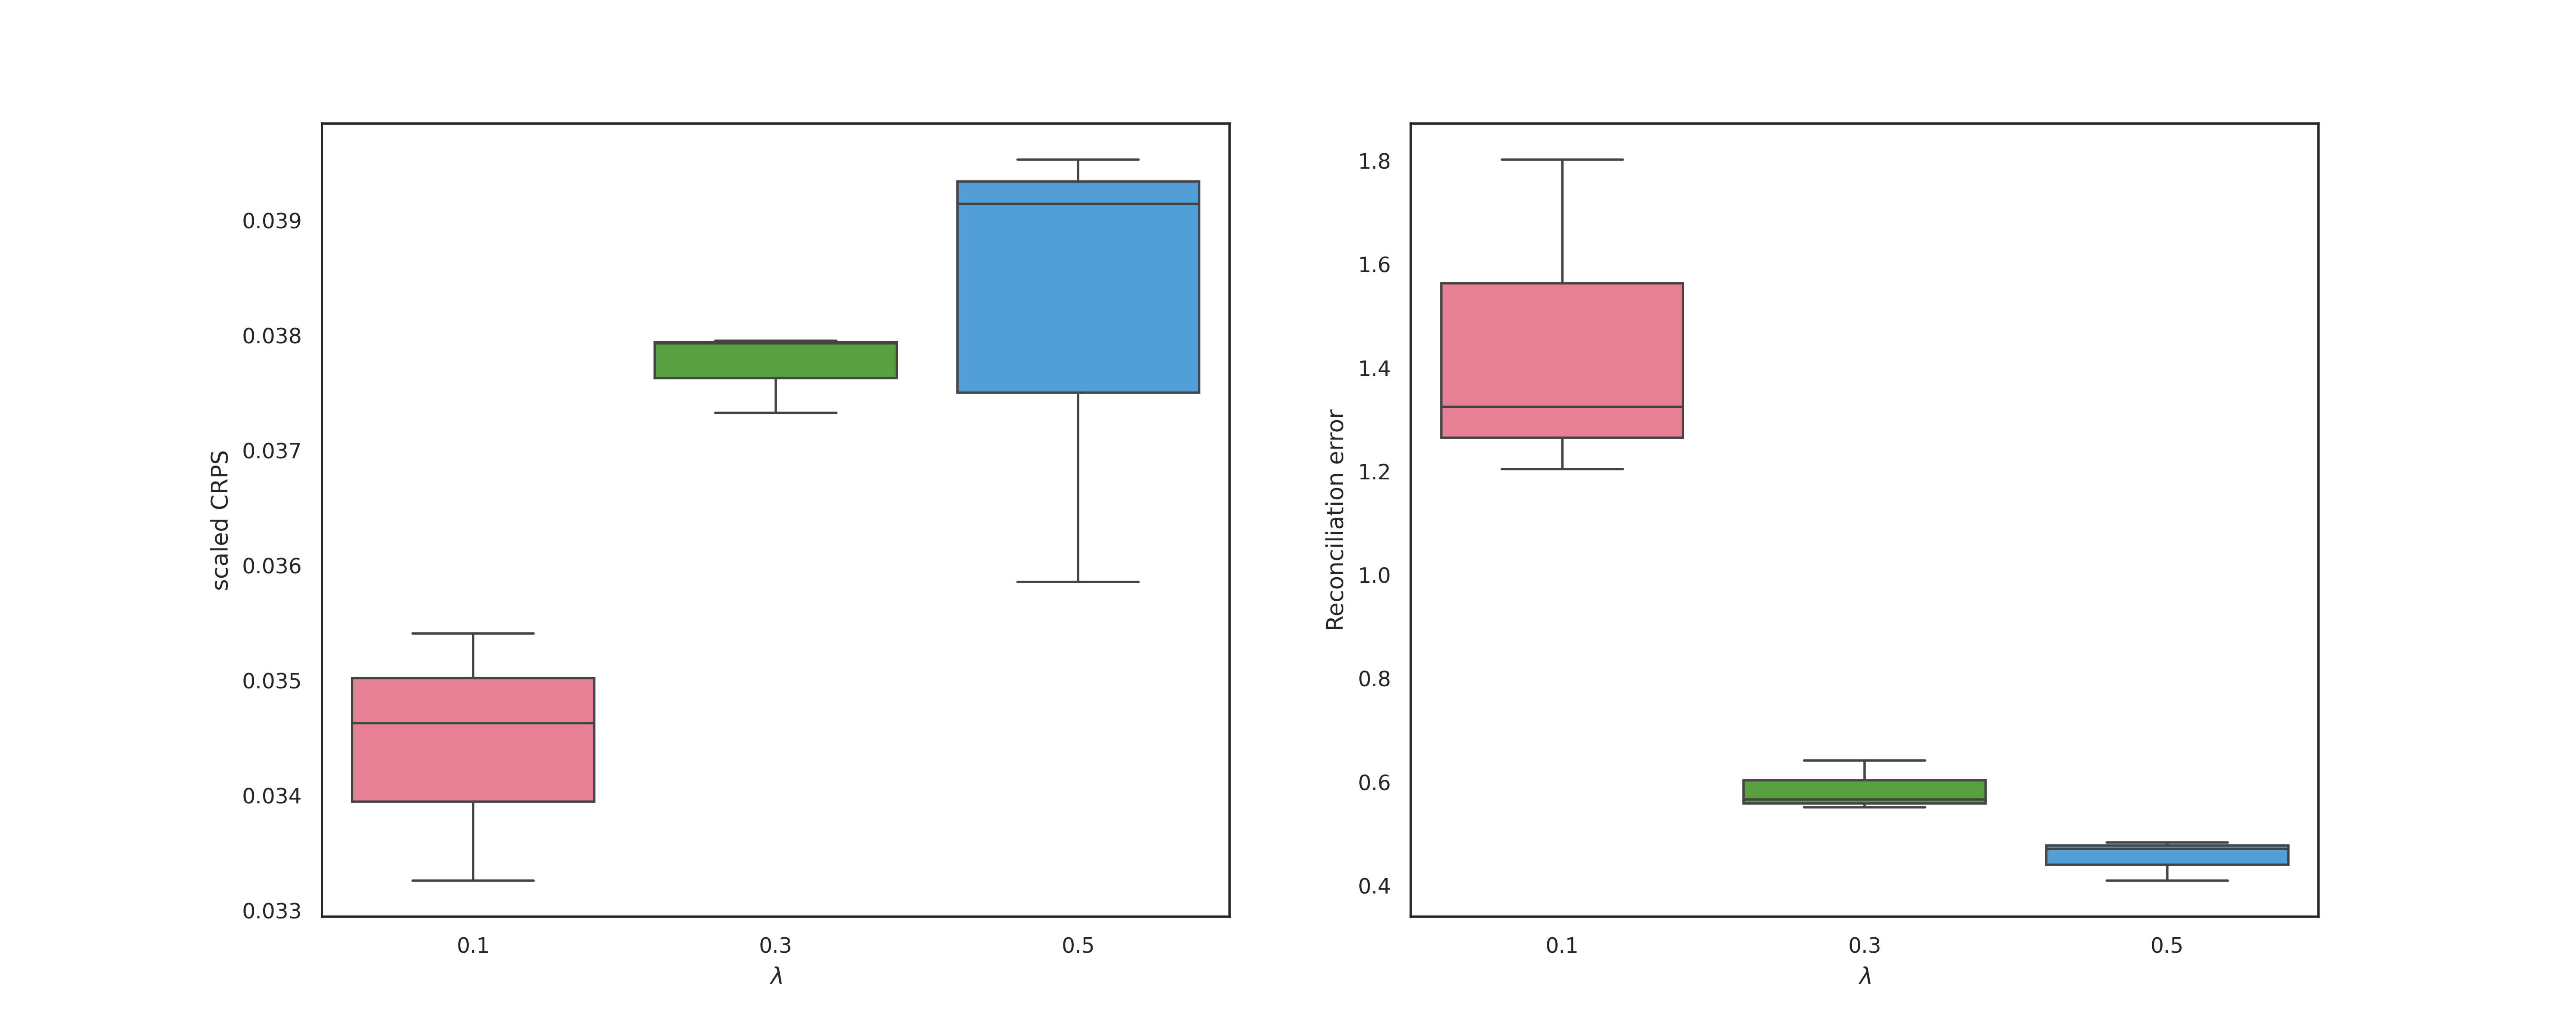
\includegraphics[width=\linewidth]{reconciliation_error.png}
    \caption{Box-plot of five independent runs of PROFHIT model. $\lambda$ is the regularization parameter enforcing coherence. The first plot shows the performance(scaled CRPS averaged over the hierarchy) while the second shows the coherence (average of the symmetrized KL divergence over the dataset)}
    \label{fig:PROFHIT}
\end{figure*}

This result suggests that the PROFHIT model, in its current form, struggles to effectively leverage hierarchical information on our dataset. 
Instead of serving as a beneficial structural prior, the regularization term for aggregation coherence introduces an additional optimization objective. 
Rather than simplifying the learning landscape, this added dimension appears to complicate model training, 
ultimately confusing the learning dynamics and impeding convergence to more accurate forecasts.

It is also worth noting that our dataset is characterized by a strictly enforced hierarchical structure—aggregation constraints are satisfied exactly by construction. 
As a result, the inherent flexibility of PROFHIT, which is designed to accommodate approximate or soft hierarchies, remains unexploited in our setting. 
Empirically, we find that our problem favors a reconciliation-based approach, 
where forecasts are first generated and then adjusted post-hoc to ensure consistency, over the PROFHIT regularization paradigm, 
in which coherence is integrated directly into the learning objective.

In summary, the combination of strict hierarchical consistency in the data and suboptimal trade-offs between coherence and predictive skill make PROFHIT ill-suited as a principal forecasting model for this application.

\subsection{Evaluation of HierE2E and CLOVER Architectures}

We next evaluate the HierE2E and CLOVER architectures. 
Our results indicate a substantial improvement in performance when these hierarchical frameworks are combined with the modern NBEATS and NHITS forecasting networks, as compared to their originally proposed neural components (MQCNN for CLOVER and DeepAR for HierE2E). 
This confirms that the choice of underlying forecasting model is critical, especially given the limitations of our dataset (see table \ref{tab:backbones}).

For the HierE2E framework, we find that the use of the default coherence enforcement, which is based on projection, yields inferior results— even below the performance of the unreconciled (incoherent) setting (table \ref{tab:recon}). 
We attribute this underperformance to the fact that the projection operation can mix signals from nodes with very different amplitudes, which appears to confuse the model with respect to the calibration of predictive uncertainty intervals. 
In contrast, when we employ a straightforward bottom-up reconciliation within the HierE2E framework, we observe not only a significant uplift relative to the standard HierE2E architecture but also improved performance when compared to the architecture without any reconciliation. 
This highlights the importance of selecting appropriate reconciliation techniques, tailored to the idiosyncrasies of the underlying data structure. 
Furthermore, this result confirms that the performance reconciliation tradeoff observed with the PROFHIT model was an artifact of the architecture and not a feature of the dataset itself. 

Turning to CLOVER, our experiments reveal optimal results when the rank of the factor model used for covariance estimation is set to five. 
Empirically, the model does not benefit from increasing the rank further, suggesting a limited ability to capture a richer or more complex covariance structure. 
This is likely a consequence of the restricted sample size and the inherently noisy estimation of cross-series relationships. 
The CLOVER framework appears to model only sparse residual dependencies beyond individual variances under these data constraints.

For both CLOVER and HierE2E, we conduct an ablation study to assess the impact of sectoral disaggregation alongside the geographical hierarchy (figure \ref{fig:improvement}). 
Specifically, we compare model performance on a purely geographical hierarchy to that obtained when sector-level disaggregation is introduced. 
Results indicate that CLOVER benefits more markedly from the expansion in the number of time series, especially at the regional level, where performance increases substantially. 
For both architectures, however, there is a modest decline in accuracy at the macro-region level, possibly reflecting increased difficulty in reconciling fine-grained information with higher-level aggregates.

In summary, the combination of advanced forecasting architectures with appropriately chosen reconciliation strategies yields clear benefits, and the response of each framework to increased hierarchy complexity offers useful insights into their respective strengths and weaknesses.

\begin{figure*}
    \centering
    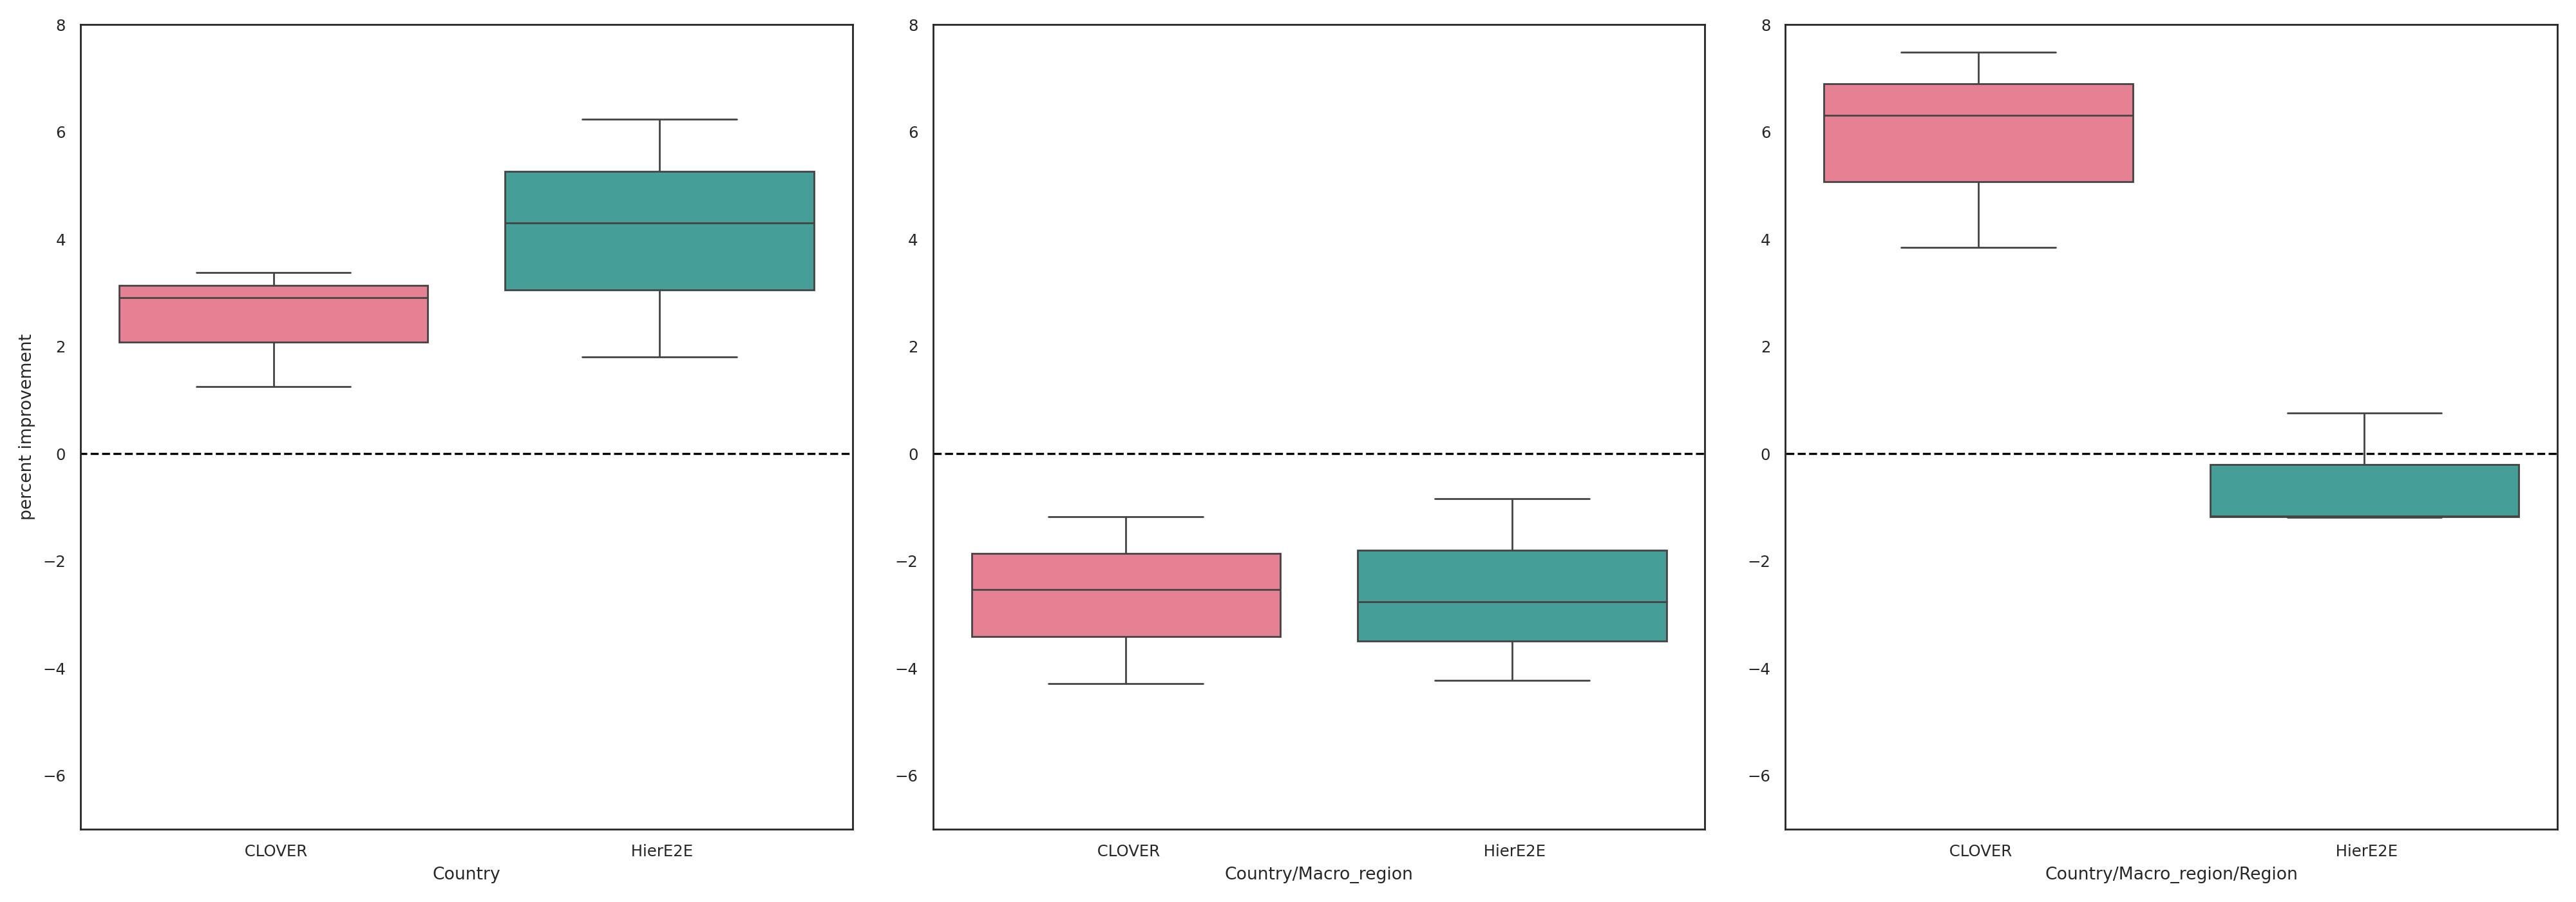
\includegraphics[width=\linewidth]{pct_improvement_sector.png}
    \caption{Percent improvement (from the addition of sector hierarchy) at each level of the geographical hierarchy. The improvement for each run is compared to the average of all runs without the sector hierarchy.}
    \label{fig:improvement}
\end{figure*}


\subsection{Benchmarking Against Standard Forecasting Methods}

To contextualize the performance of the studied hierarchical probabilistic frameworks, we benchmark our models against widely used statistical and machine learning forecasting approaches. 
Specifically, we include as relevant baselines (i) univariate ARIMA models, and (ii) neural forecasting models based on the NBEATS and NHITS architectures. 
This enables us to compare results not only against established statistical methodologies but also against state-of-the-art machine learning models that are agnostic to hierarchical structure.

For each baseline model, we additionally assess forecast performance when traditional reconciliation techniques are applied. 
In particular, we consider both the bottom-up and MinTrace methods, allowing us to isolate the marginal contribution of classical post-hoc reconciliation relative to the studied end-to-end frameworks. 
Empirically, we find that the bootstrapping-based probabilistic reconciliation method yields consistently better results than the PERMBU variant; therefore, all reported results in this study utilize the former.

In the case of ARIMA, the probabilistic cumulative distribution function is constructed via conformal prediction, which provides the quantile estimates required for CRPS computation. 
For the NBEATS and NHITS models, we use parametric Gaussian predictive distributions, implemented identically to those in our end-to-end frameworks to ensure fair comparability of probabilistic metrics.

This comprehensive benchmarking strategy enables us to (i) quantify the benefit of advanced end-to-end hierarchical modeling over traditional approaches, 
and (ii) disentangle gains attributable to the core forecasting model from those stemming from hierarchical reconciliation procedures.

Our results are presented in Tables~\ref{tab:benchmarksCRPS},~\ref{tab:benchmarksSMAPE} and in Figure~\ref{fig:benchmarkplots} for ease of interpretation. 
The results demonstrate that the proposed hierarchical models yield substantial improvements in probabilistic forecasting accuracy over standard benchmarks. 
Specifically, the studied end-to-end frameworks achieve a mean reduction in scaled CRPS of approximately 35\% relative to univariate ARIMA, 18\% relative to reconciled ARIMA, and around 14\% with respect to neural network approaches using NBEATS and NHITS as standalone forecasters. 
These gains are consistent across all levels of the hierarchy and are particularly pronounced at the lowest levels, which correspond to the most challenging time series from a forecasting perspective. 
This indicates that leveraging the hierarchical structure in an end-to-end manner enables the model to more effectively share information across related series, thus enhancing predictive performance where signals are the noisiest and hardest to predict.

Additionally, we observe that the HierE2E and CLOVER frameworks display broadly comparable results across most levels of the hierarchy, with the exception of the region level, where CLOVER outperforms HierE2E by a margin of roughly 5\%. 
This advantage is likely attributable to CLOVER’s explicit modeling of cross-series dependencies through its covariance structure. 
However, the overall effect remains moderate, consistent with our earlier findings that the low-rank constraint (five latent factors) limits the capacity of the covariance estimator to capture more nuanced inter-series relationships. 
This further underscores the trade-off between sample size and complexity in learning multivariate dependencies within hierarchical time series data.


\section{Conclusion and Perspectives}

In this study, we provide a comprehensive methodological and empirical evaluation of modern end-to-end probabilistic forecasting frameworks for hierarchical time series, with a focused application to the challenging domain of Italian private debt markets. 
Our work bridges the gap between recent advances in deep learning-based probabilistic forecasting and the practical requirements of coherent, scale-robust aggregation found in financial hierarchies.

We analyze three state-of-the-art frameworks---PROFHIT, HierE2E, and CLOVER---and benchmark their performance against both classical (ARIMA) and machine learning (NBEATS, NHITS) approaches, including traditional reconciliation strategies such as bottom-up and MinTrace. 
Our results reveal several key insights:


First, our findings indicate that both the forecasting architecture and choice of reconciliation method are critical to effective performance. 
PROFHIT’s regularization-based coherence enforcement appears less effective on datasets with strict aggregation and modest sample sizes, 
while direct reconciliation---especially via bottom-up strategies---within HierE2E and CLOVER offers superior coherence without the performance trade-off observed in regularization approaches. 
Additionally, CLOVER’s explicit modeling of cross-series dependencies provides advantages at intermediate aggregation levels, though its benefits over simpler architectures are modest, reflecting practical limits imposed by data sparsity on covariance estimation.

Second, evidence both from QQ plots analysis and the observed empirical performance justifies the Gaussian assumption for predictive distributions in credit aggregates, 
given the maintained level of aggregation, but also indicate potential avenues for further research into heavy-tailed phenomena at the lowest levels,
 especially in the optic of extending the dataset to more granular levels (such as province level signals). 

Finally, our benchmarking demonstrates that advanced hierarchy-aware methods achieve a reduction of up to 35\% in scaled CRPS compared to classical ARIMA, 
and 14--18\% compared to unreconciled and classically reconciled neural models, 
substantiating the value of end-to-end hierarchical methodologies in real-world probabilistic forecasting tasks. 

We further show that the benefits of the end-to-end reconciliation approach are most pronounced at the lowest,
noisiest levels of the aggregation hierarchy. 
Here, leveraging the natural structure encoded in the hierarchy allows the studied frameworks to significantly outperform both unreconciled and classically reconciled benchmarks, 
most notably in probabilistic evaluation, but also with respect to point forecast accuracy.

\textbf{Perspectives.} While this study demonstrates the robustness and adaptability of end-to-end neural reconciliation for private debt applications, it also highlights future directions. 

A promising direction for future research is the exploration of heavy-tailed and non-Gaussian processes at the most disaggregated levels of the hierarchy. 
For more granular hierarchical representations, the use of mixed parametric distribution models, such as those implemented in the HAILS framework \cite{HAILS}, may be required to maintain forecast accuracy. 
However, an important challenge lies in appropriately modeling the sparse and irregular nature of loan origination or default events. 
Unlike retail sales data, which can often be effectively modeled using Poisson count distributions, the generative process underlying loan origination may not conform to standard discrete or waiting-time distributions. 
Careful investigation into the statistical properties and suitable probabilistic models for such sparse financial events is thus essential for the advancement of probabilistic forecasting at finer hierarchical levels.

Another promising avenue for future research lies in the use of clustering techniques to construct intermediate-level time series within hierarchical structures. 
Recent work by Zhang et al.\cite{cluster} demonstrates that designing hierarchies based on clustering—rather than relying solely on pre-defined, domain-driven groupings—can lead to improvements in forecast accuracy. 
Their results, however, are derived primarily from benchmark datasets, such as Australian tourism, which are characterized by pronounced trends and strong seasonal temporal correlations. 
Extending this clustering-based approach to the credit domain constitutes an interesting direction, particularly given the more modest predictability and lower degree of seasonality typically present in financial time series. 
Furthermore, integrating data-driven hierarchy construction within end-to-end probabilistic forecasting frameworks may offer additional gains, effectively combining the strengths of hierarchical reconciliation and automated structure learning.

Lastly, while significant progress has been made in the development of end-to-end probabilistic architectures for hierarchical and grouped time series, 
existing frameworks have yet to be extended, to the best of our knowledge, to accommodate temporal or cross-temporal hierarchies. 
In the context of debt, for example, one could naturally construct a temporal hierarchy by including origination data at quarterly and yearly reporting frequencies alongside the monthly series. 
Leveraging such cross-temporal structures offers the potential for further improvements in both forecast accuracy and coherence, and represents an important and largely unexplored direction for future research in probabilistic time series forecasting.

\section{Acknowledgments}

This study has been conducted as part of the MSCA DIGITAL project.
This project has received funding from the Horizon Europe research and innovation programme under the Marie Skłodowska-Curie Grant Agreement No. 101119635.

\begin{figure}[h]
    \centering
    
\includegraphics[width=\linewidth]{EU_fund.jpg}
\end{figure}

\section{Note on reproducibility}

To ensure transparency and reproducibility, all codes, trained models, 
and data preprocessing scripts used in this study are made publicly available as part of the Q2 (Quantinar-Quantlet) ecosystem.

Minimal working examples are provided in the Quantlet format, 
facilitating straightforward replication and extension of our results. 
The complete repository can be found at: \url{https://github.com/QuantLet/Hierarchical-Loan-Forecasting/tree/main}

This commitment to open science in alignment with the terms of the Marie Skłodowska-Curie Grant Agreement No. 101119635 and supports both the verification of our findings and the advancement of further research.

\begin{figure*}
    \centering
     \begin{subfigure}[b]{\textwidth}
         \centering
         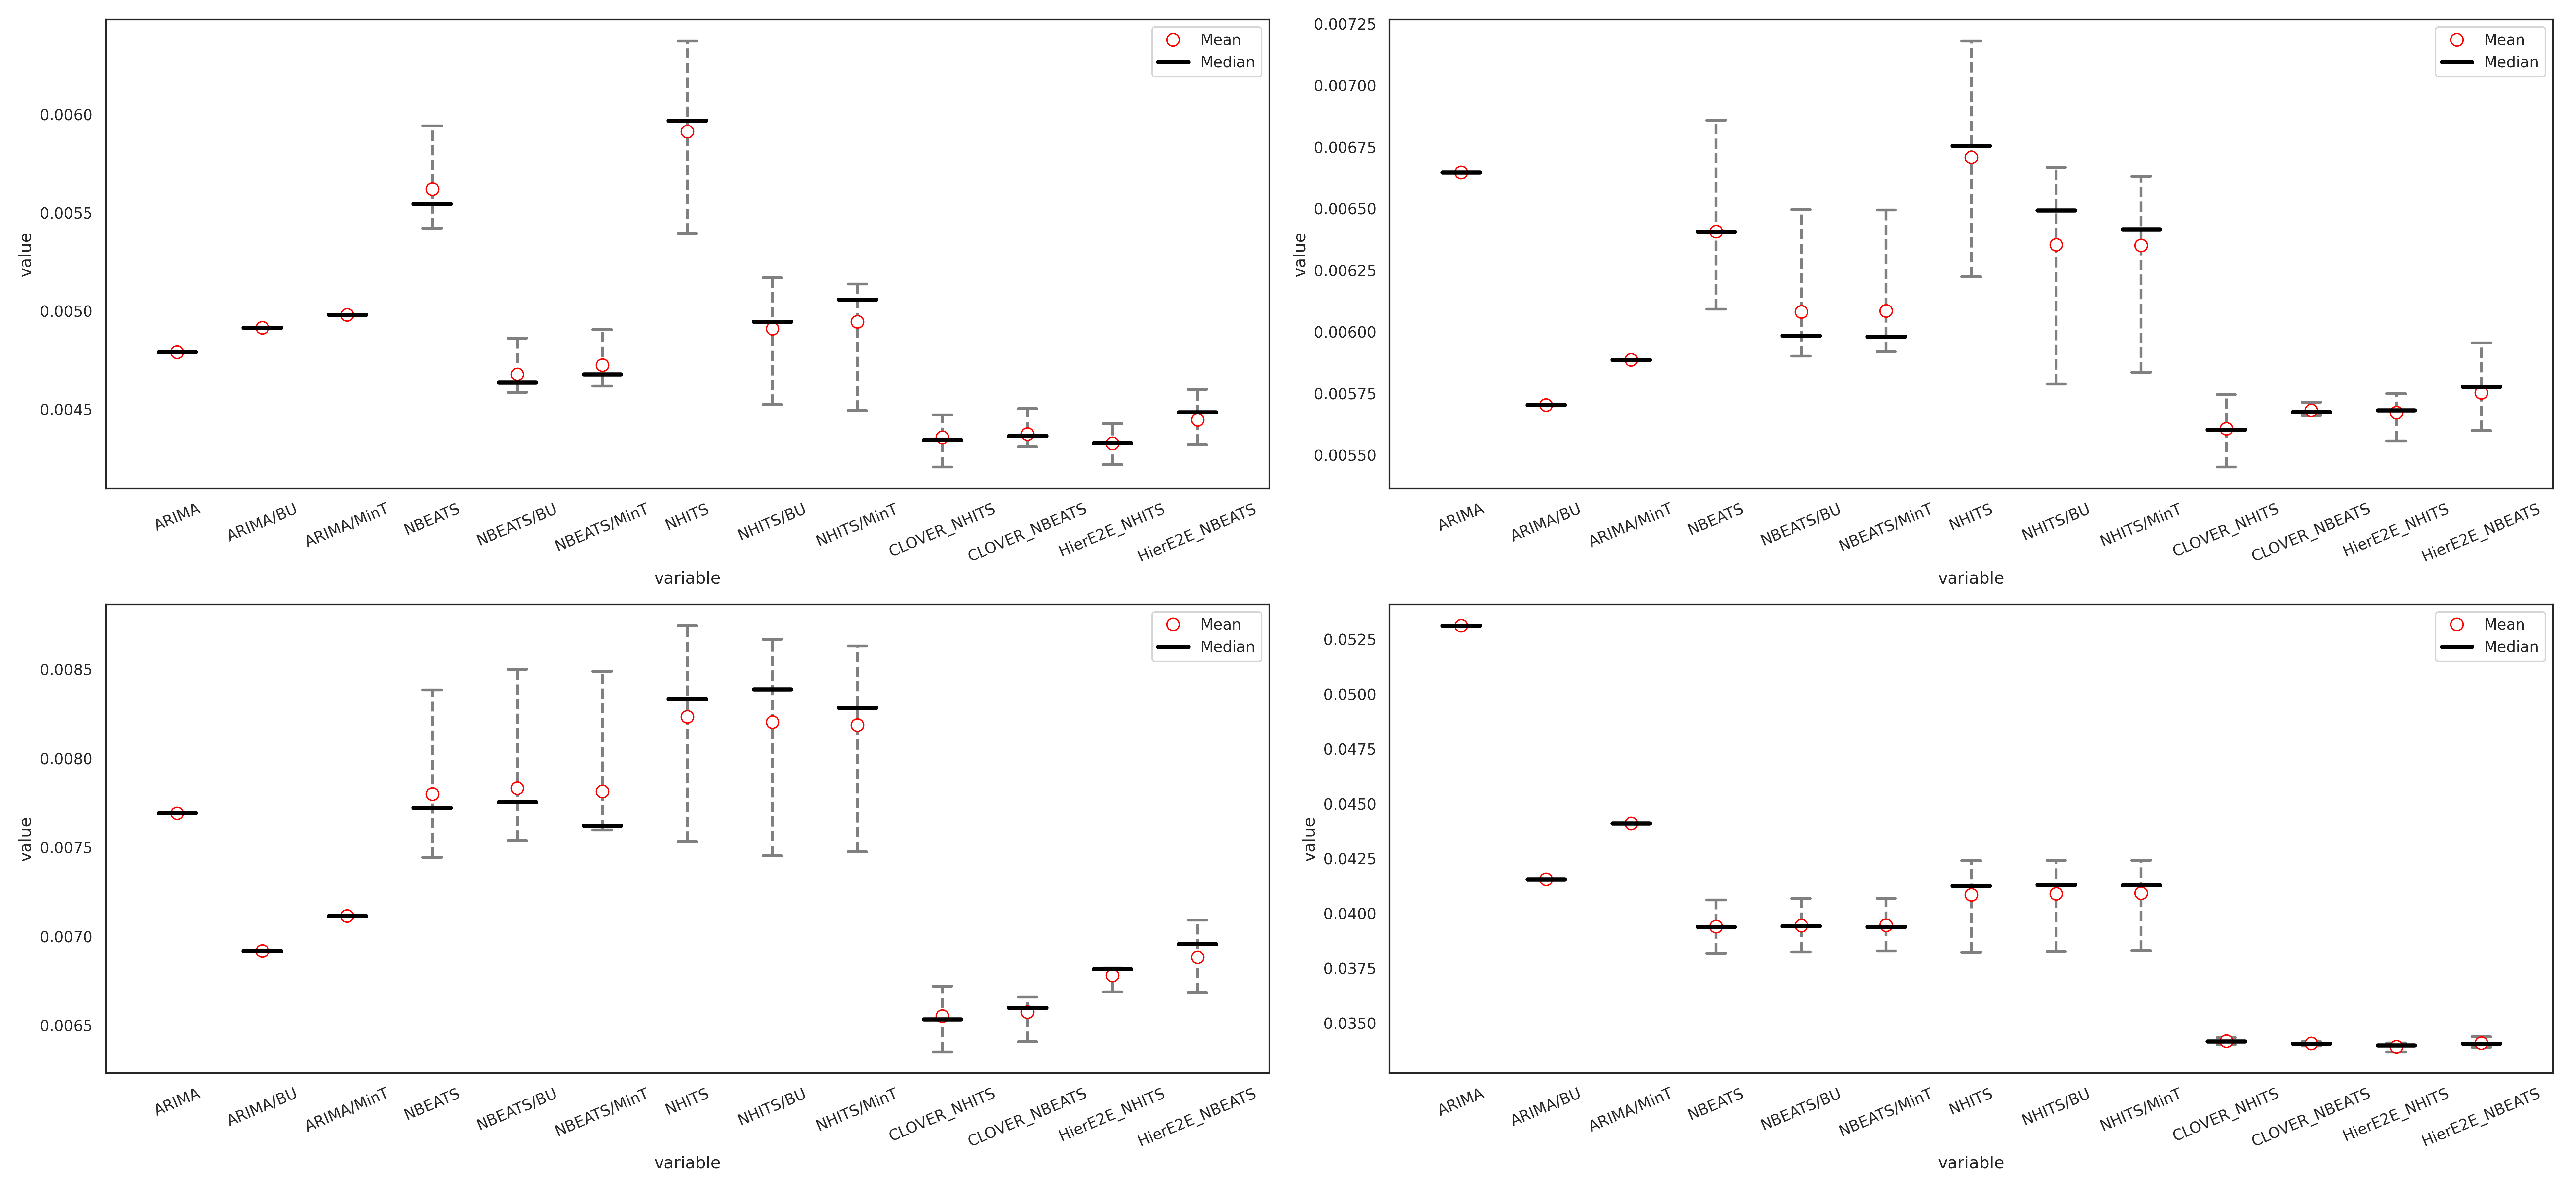
\includegraphics[width=\textwidth]{minmax_benchmark_CRPS.png}
         \caption{Scaled CRPS at each hierarchical level.}
         \label{fig:benchsub1}
     \end{subfigure}
     \begin{subfigure}[b]{\textwidth}
         \centering
         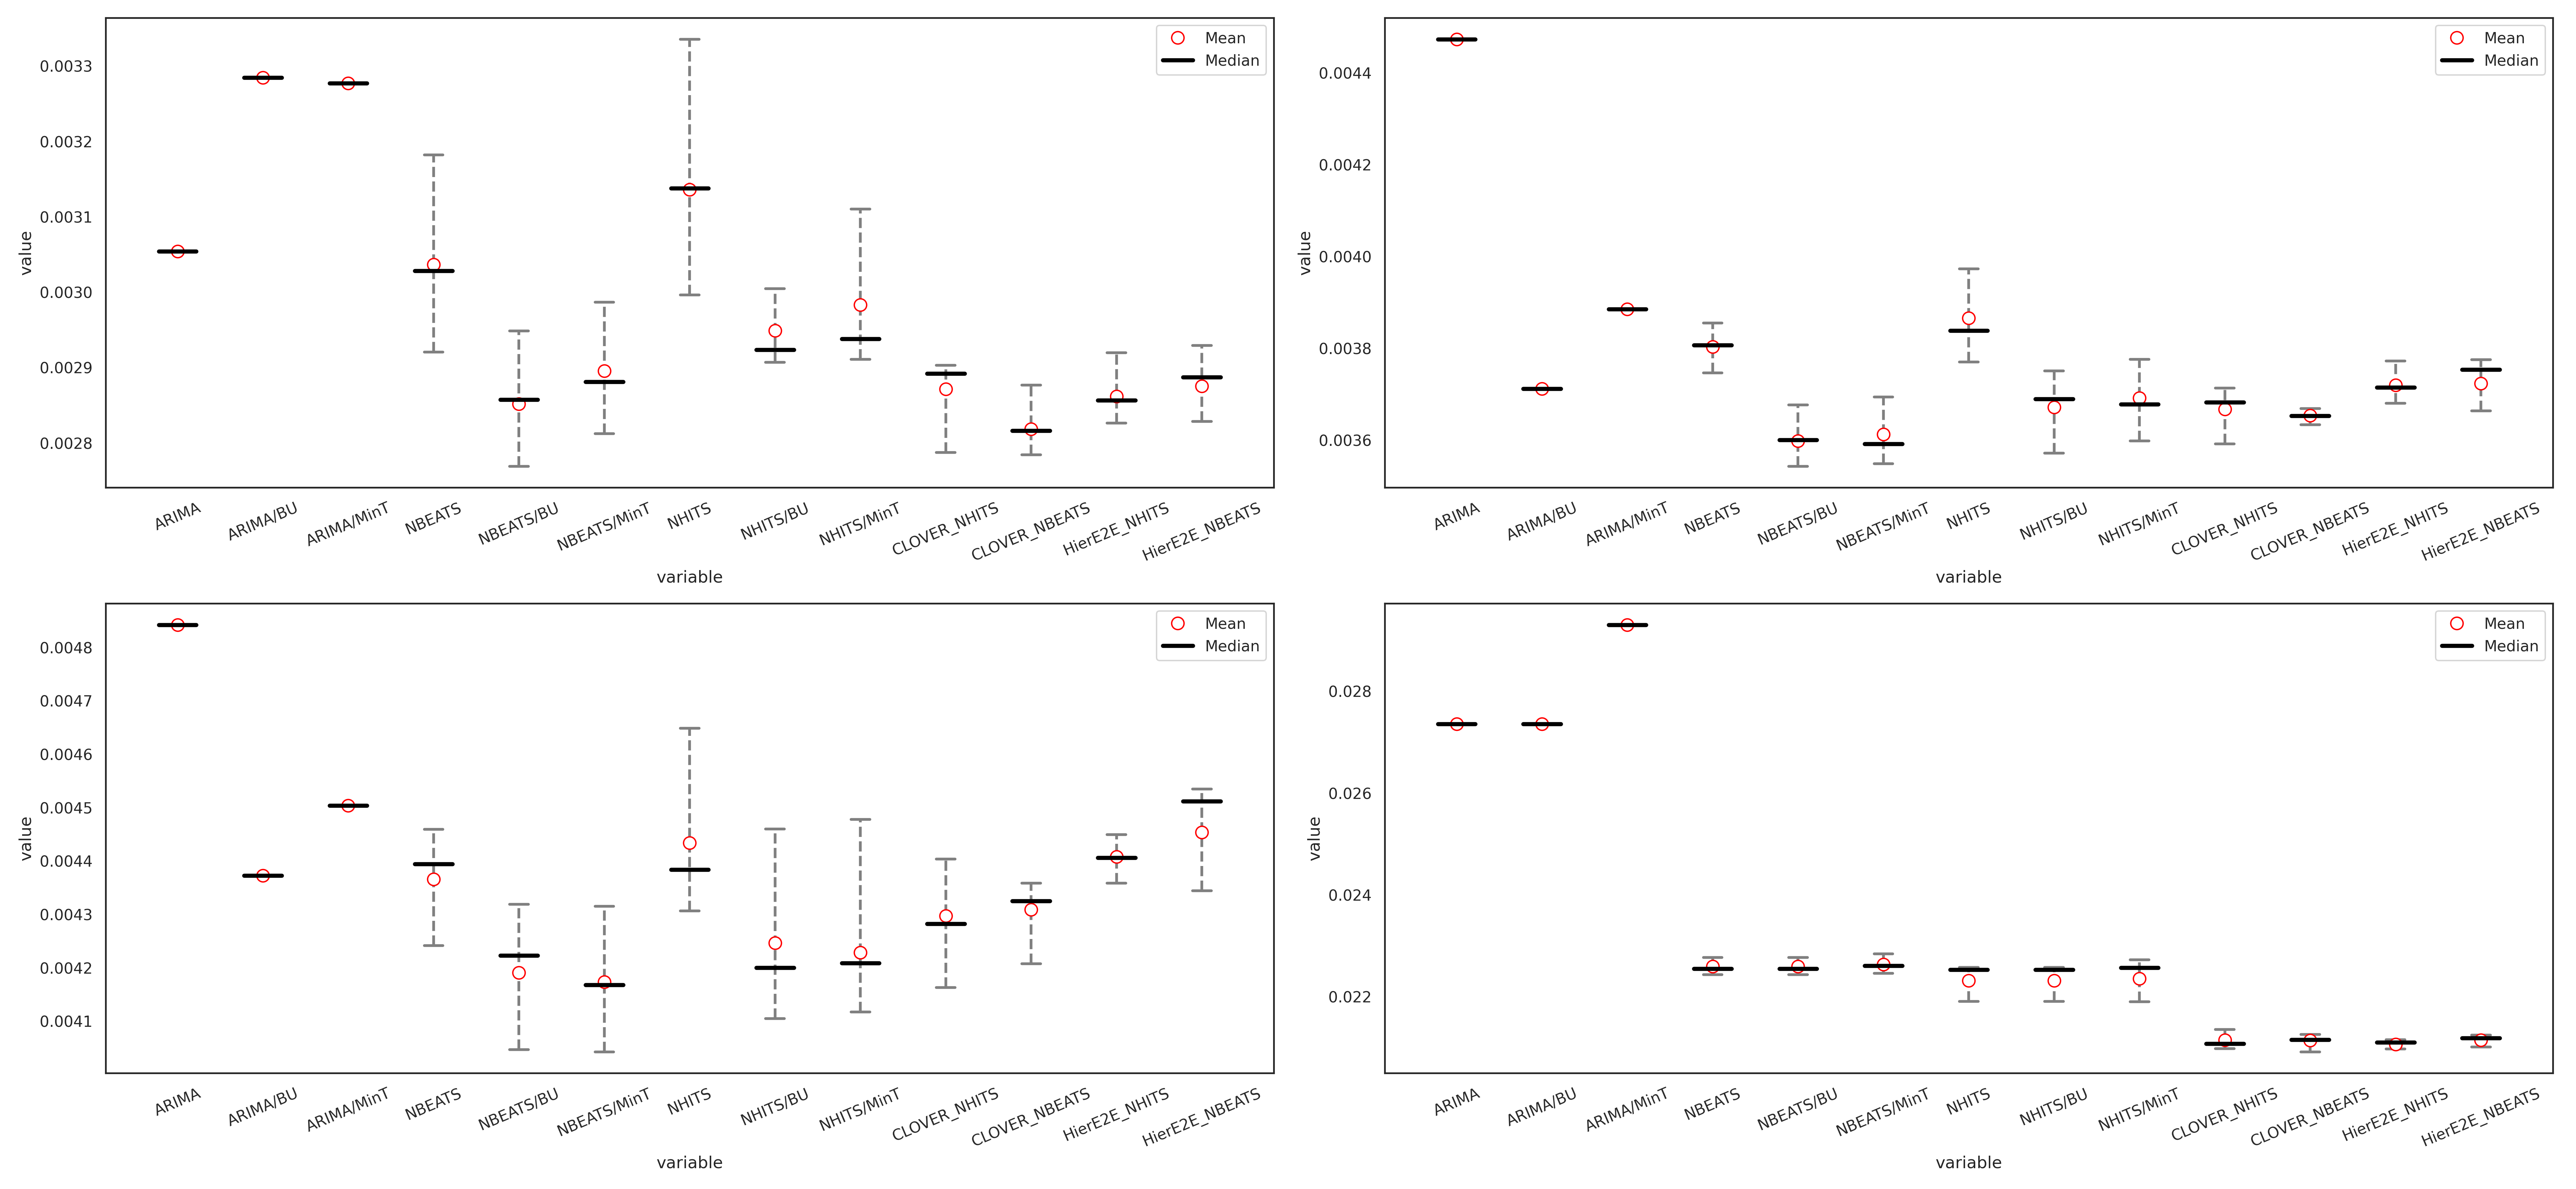
\includegraphics[width=\textwidth]{minmax_benchmark_SMAPE.png}
         \caption{SMAPE at each hierarchical level.}
         \label{fig:benchsub2}
     \end{subfigure}
     \hfill
        \caption{
Plots of model performance (lower is better) for the studied hierarchical probabilistic models, and benchmark neural network and statistical (ARIMA) approaches. Performance is shown at each level of the hierarchy, including the mean, median and min-max interval over 5 independent runs, except ARIMA where results are invariant across runs. 
}
    \label{fig:benchmarkplots}
\end{figure*}



\begin{table*}[h]
    \centering
    \resizebox{\textwidth}{!}{%
    {
\renewcommand{\arraystretch}{1.2}

\renewcommand{\textbf}[1]{\color{red}\bfseries #1}
\renewcommand{\underline}[1]{\color{blue}\uline{#1}}

    \begin{tabular}{llllllll}
\toprule
level & metric & HierE2E NHITS & HierE2E NBEATS & HierE2E DeepAR & CLOVER NHITS & CLOVER NBEATS & CLOVER MQCNN \\
\midrule
Country & scaled crps & \textbf{0.0043 ± 0.0001} & 0.0044 ± 0.0001 & 0.0048 ± 0.0004 & \underline{0.0044 ± 0.0001} & 0.0044 ± 0.0001 & 0.0088 ± 0.0023 \\
Country & smape & \underline{0.0029 ± 0.0000} & 0.0029 ± 0.0000 & 0.0031 ± 0.0002 & 0.0029 ± 0.0000 & \textbf{0.0028 ± 0.0000} & 0.0053 ± 0.0013 \\
Country & mase & \underline{0.5256 ± 0.0060} & 0.5282 ± 0.0074 & 0.5636 ± 0.0394 & 0.5268 ± 0.0084 & \textbf{0.5175 ± 0.0061} & 0.9753 ± 0.2348 \vspace{0.2em}\\
\hline \vspace{-0.9em} \\
Macro region & scaled crps & \underline{0.0057 ± 0.0001} & 0.0058 ± 0.0001 & 0.0061 ± 0.0004 & \textbf{0.0056 ± 0.0001} & 0.0057 ± 0.0000 & 0.0091 ± 0.0020 \\
Macro region & smape & 0.0037 ± 0.0000 & 0.0037 ± 0.0001 & 0.0040 ± 0.0002 & \underline{0.0037 ± 0.0000} & \textbf{0.0037 ± 0.0000} & 0.0058 ± 0.0010 \\
Macro region & mase & 0.4457 ± 0.0040 & 0.4463 ± 0.0065 & 0.4892 ± 0.0242 & \underline{0.4398 ± 0.0066} & \textbf{0.4380 ± 0.0019} & 0.6865 ± 0.1119 \vspace{0.2em}\\
\hline \vspace{-0.9em} \\

Region & scaled crps & 0.0068 ± 0.0001 & 0.0069 ± 0.0002 & 0.0075 ± 0.0005 & \textbf{0.0066 ± 0.0001} & \underline{0.0066 ± 0.0001} & 0.0110 ± 0.0017 \\
Region & smape & 0.0044 ± 0.0000 & 0.0045 ± 0.0001 & 0.0050 ± 0.0003 & \textbf{0.0043 ± 0.0001} & \underline{0.0043 ± 0.0001} & 0.0073 ± 0.0009 \\
Region & mase & 0.4930 ± 0.0041 & 0.4986 ± 0.0093 & 0.5667 ± 0.0354 & \textbf{0.4806 ± 0.0102} & \underline{0.4828 ± 0.0058} & 0.8338 ± 0.1000 \vspace{0.2em}\\
\hline \vspace{-0.9em} \\

Sector & scaled crps & \textbf{0.0339 ± 0.0002} & 0.0341 ± 0.0002 & 0.0375 ± 0.0002 & 0.0342 ± 0.0001 & \underline{0.0341 ± 0.0001} & 0.0473 ± 0.0034 \\
Sector & smape & \textbf{0.0211 ± 0.0001} & 0.0212 ± 0.0001 & 0.0240 ± 0.0001 & 0.0212 ± 0.0001 & \underline{0.0211 ± 0.0001} & 0.0316 ± 0.0020 \\
Sector & mase & 0.6220 ± 0.0032 & 0.6214 ± 0.0023 & 0.7243 ± 0.0099 & \underline{0.6195 ± 0.0047} & \textbf{0.6184 ± 0.0033} & 0.9616 ± 0.0430 \vspace{0.2em}\\
\hline \vspace{-0.9em} \\
Overall & scaled crps & \textbf{0.0283 ± 0.0001} & 0.0284 ± 0.0002 & 0.0312 ± 0.0003 & 0.0284 ± 0.0001 & \underline{0.0283 ± 0.0001} & 0.0397 ± 0.0029 \\
Overall & smape & \textbf{0.0176 ± 0.0001} & 0.0177 ± 0.0001 & 0.0200 ± 0.0001 & 0.0176 ± 0.0001 & \underline{0.0176 ± 0.0001} & 0.0265 ± 0.0016 \\
Overall & mase & 0.5938 ± 0.0033 & 0.5942 ± 0.0035 & 0.6887 ± 0.0145 & \underline{0.5896 ± 0.0056} & \textbf{0.5889 ± 0.0036} & 0.9305 ± 0.0530 \\
\bottomrule
\end{tabular}    
    }}
    \caption{
        Performance evaluation of the HierE2E and CLOVER frameworks across different neural network forecasting backbones. Results are reported as the mean and standard deviation aggregated over five independent runs. The best (lowest) scores for each metric and hierarchy level are highlighted in bold. Metrics are provided at every level of the hierarchy, including both probabilistic (scaled CRPS) and point-forecast metrics (sMAPE and MASE), all of which are scale-invariant. All models are trained using the optimal hyperparameters found for each configuration. Note that the DeepAR-HierE2E combination reflects the best-performing reconciliation method identified in this study and may differ from the original implementation proposed in the HierE2E paper, as the paper's method was found to be suboptimal in our experimental setting.
        }
    \label{tab:backbones}
\end{table*}


\begin{table*}
    \centering
    \resizebox{\textwidth}{!}{%
    {
\renewcommand{\arraystretch}{1.2}
\renewcommand{\textbf}[1]{\color{red}\bfseries #1}
\renewcommand{\underline}[1]{\color{blue}\uline{#1}}
    \begin{tabular}{lllll}
\toprule
level & metric & HierE2E/Bottom-Up & HierE2E/No reconciliation & HierE2E/Projection \\
\midrule
Country & scaled crps & \textbf{0.0043 ± 0.0001} & \underline{0.0051 ± 0.0001} & 0.6899 ± 0.0819 \\
Country & smape & \textbf{0.0029 ± 0.0000} & \underline{0.0033 ± 0.0001} & 0.5866 ± 0.1059 \\
Country & mase & \textbf{0.5249 ± 0.0059} & \underline{0.6020 ± 0.0135} & 66.7718 ± 8.7611 \vspace{0.2em} \\
\hline \vspace{-0.9em} \\
Macro region & scaled crps & \textbf{0.0057 ± 0.0001} & \underline{0.0061 ± 0.0001} & 0.6202 ± 0.0172 \\
Macro region & smape & \textbf{0.0037 ± 0.0000} & \underline{0.0040 ± 0.0001} & 0.5402 ± 0.0208 \\
Macro region & mase & \textbf{0.4457 ± 0.0040} & \underline{0.4755 ± 0.0090} & 42.5062 ± 0.5819 \\
\hline \vspace{-0.9em} \\
Region & scaled crps & \textbf{0.0068 ± 0.0001} & \underline{0.0073 ± 0.0001} & 0.8273 ± 0.0240 \\
Region & smape & \textbf{0.0044 ± 0.0000} & \underline{0.0047 ± 0.0001} & 0.5694 ± 0.0160 \\
Region & mase & \textbf{0.4931 ± 0.0041} & \underline{0.5234 ± 0.0104} & 54.3537 ± 2.0333 \vspace{0.2em} \\
\hline \vspace{-0.9em}\\
Sector & scaled crps & \textbf{0.0339 ± 0.0002} & \underline{0.0340 ± 0.0000} & 22.1841 ± 3.6263 \\
Sector & smape & \underline{0.0211 ± 0.0001} & \textbf{0.0210 ± 0.0001} & 0.8204 ± 0.0055 \\
Sector & mase & \underline{0.6220 ± 0.0032} & \textbf{0.6210 ± 0.0036} & 313.4676 ± 41.1283 \vspace{0.2em} \\
\hline \vspace{-0.9em} \\
Overall & scaled crps & \textbf{0.0283 ± 0.0001} & \underline{0.0284 ± 0.0000} & 17.7678 ± 2.8824 \\
Overall & smape & \textbf{0.0176 ± 0.0001} & \underline{0.0176 ± 0.0000} & 0.7676 ± 0.0067 \\
Overall & mase & \textbf{0.5938 ± 0.0033} & \underline{0.5996 ± 0.0045} & 259.6281 ± 33.0103 \\
\bottomrule
\end{tabular}
}}
\caption{
Performance evaluation of the HierE2E framework using different hierarchical reconciliation methods. The projection-based reconciliation yields substantially poorer results, with evidence of non-convergence during training. In contrast, applying bottom-up reconciliation leads to consistently superior performance compared to unreconciled models at all hierarchical levels, with pronounced improvements observed for aggregated nodes. Metrics are reported as mean and standard deviation over five independent runs.}
    \label{tab:recon}
\end{table*}









\begin{table*}[h]
    \centering 
    \resizebox{\textwidth}{!}{%
    {
\renewcommand{\arraystretch}{1.2}
\renewcommand{\textbf}[1]{\color{red}\bfseries #1}
\renewcommand{\underline}[1]{\color{blue}\uline{#1}}
       \begin{tabular}{llllll}
\toprule
Hierarchy Level & Country & Macro region & Region & Sector & Overall \\
\midrule
ARIMA & 0.004792 & 0.006647 & 0.007693 & 0.053130 & 0.043690 \\
ARIMA/BottomUp & 0.004917 & 0.005705 & 0.006919 & 0.041565 & 0.034352 \\
ARIMA/MinTrace & 0.004982 & 0.005888 & 0.007117 & 0.044115 & 0.036415 \vspace{0.2em} \\ 
\hline  \vspace{-0.9em} \\ 
NBEATS & 0.0056 ± 0.0002 & 0.0064 ± 0.0003 & 0.0078 ± 0.0003 & 0.0394 ± 0.0008 & 0.0328 ± 0.0007 \\
NBEATS/BottomUp & 0.0047 ± 0.0001 & 0.0061 ± 0.0002 & 0.0078 ± 0.0004 & 0.0395 ± 0.0008 & 0.0328 ± 0.0007 \\
NBEATS/MinTrace & 0.0047 ± 0.0001 & 0.0061 ± 0.0002 & 0.0078 ± 0.0003 & 0.0395 ± 0.0008 & 0.0328 ± 0.0007 \\
NHITS & 0.0059 ± 0.0003 & 0.0067 ± 0.0003 & 0.0082 ± 0.0004 & 0.0409 ± 0.0014 & 0.0341 ± 0.0012 \\
NHITS/BottomUp & 0.0049 ± 0.0002 & 0.0064 ± 0.0003 & 0.0082 ± 0.0004 & 0.0409 ± 0.0014 & 0.0341 ± 0.0012 \\
NHITS/MinTrace & 0.0049 ± 0.0002 & 0.0064 ± 0.0003 & 0.0082 ± 0.0004 & 0.0409 ± 0.0014 & 0.0341 ± 0.0012 \vspace{0.2em} \\
\hline \vspace{-0.9em} \\ 
CLOVER NHITS & \underline{0.0044 ± 0.0001} & \textbf{0.0056 ± 0.0001} & \textbf{0.0066 ± 0.0001} & 0.0342 ± 0.0001 & 0.0284 ± 0.0001 \\
CLOVER NBEATS & 0.0044 ± 0.0001 & 0.0057 ± 0.0000 & \underline{0.0066 ± 0.0001} & \underline{0.0341 ± 0.0001} & \underline{0.0283 ± 0.0001} \\
HierE2E NHITS & \textbf{0.0043 ± 0.0001} & \underline{0.0057 ± 0.0001} & 0.0068 ± 0.0001 & \textbf{0.0339 ± 0.0002} & \textbf{0.0283 ± 0.0001} \\
HierE2E NBEATS & 0.0044 ± 0.0001 & 0.0058 ± 0.0001 & 0.0069 ± 0.0002 & 0.0341 ± 0.0002 & 0.0284 ± 0.0002 \\
\bottomrule
\end{tabular}
    } }
    \caption{ Benchmark comparison of 
probabilistic performance of hierarchical end-to-end forecasting approaches against standard statistical and machine learning models. Results are reported for univariate ARIMA, NBEATS, and NHITS models, both with and without traditional reconciliation methods (bottom-up and MinTrace). Performance is assessed using \textbf{scaled CRPS}. Best performing model is highlighted in bold (best average performance) and second best is underlined.
}
    \label{tab:benchmarksCRPS}
\end{table*}

\begin{table*}[h]
    \centering 
    \resizebox{\textwidth}{!}{%
    {
\renewcommand{\arraystretch}{1.2}
\renewcommand{\textbf}[1]{\color{red}\bfseries #1}
\renewcommand{\underline}[1]{\color{blue}\uline{#1}}
       \begin{tabular}{llllll}
\toprule
Hierarchy Level & Country & Macro region & Region & Sector & Overall \\
\midrule
ARIMA & 0.003054 & 0.004473 & 0.004843 & 0.027361 & 0.022685 \\
ARIMA/BottomUp & 0.003285 & 0.003713 & 0.004373 & 0.027361 & 0.022582 \\
ARIMA/MinTrace & 0.003277 & 0.003886 & 0.004504 & 0.029306 & 0.024154 \vspace{0.2em}\\
\hline \vspace{-0.9em} \\
NBEATS & 0.0030 ± 0.0001 & 0.0038 ± 0.0000 & 0.0044 ± 0.0001 & 0.0226 ± 0.0001 & 0.0188 ± 0.0001 \\
NBEATS/BottomUp & \underline{0.0029 ± 0.0001} & \textbf{0.0036 ± 0.0001} & \underline{0.0042 ± 0.0001} & 0.0226 ± 0.0001 & 0.0188 ± 0.0001 \\
NBEATS/MinTrace & 0.0029 ± 0.0001 & \underline{0.0036 ± 0.0001} & \textbf{0.0042 ± 0.0001} & 0.0226 ± 0.0001 & 0.0188 ± 0.0001 \\
NHITS & 0.0031 ± 0.0001 & 0.0039 ± 0.0001 & 0.0044 ± 0.0001 & 0.0223 ± 0.0003 & 0.0186 ± 0.0002 \\
NHITS/BottomUp & 0.0029 ± 0.0000 & 0.0037 ± 0.0001 & 0.0042 ± 0.0001 & 0.0223 ± 0.0003 & 0.0186 ± 0.0002 \\
NHITS/MinTrace & 0.0030 ± 0.0001 & 0.0037 ± 0.0001 & 0.0042 ± 0.0001 & 0.0224 ± 0.0003 & 0.0186 ± 0.0003 \vspace{0.2em}\\
\hline \vspace{-0.9em} \\
CLOVER NHITS & 0.0029 ± 0.0000 & 0.0037 ± 0.0000 & 0.0043 ± 0.0001 & 0.0211 ± 0.0001 & 0.0176 ± 0.0001 \\
CLOVER NBEATS & \textbf{0.0028 ± 0.0000} & 0.0037 ± 0.0000 & 0.0043 ± 0.0001 & \underline{0.0211 ± 0.0001} & \underline{0.0176 ± 0.0001} \\
HierE2E NHITS & 0.0029 ± 0.0000 & 0.0037 ± 0.0000 & 0.0044 ± 0.0000 & \textbf{0.0211 ± 0.0001} & \textbf{0.0176 ± 0.0001} \\
HierE2E NBEATS & 0.0029 ± 0.0000 & 0.0037 ± 0.0000 & 0.0045 ± 0.0001 & 0.0212 ± 0.0001 & 0.0177 ± 0.0001 \\
\bottomrule
\end{tabular}
    } }
    \caption{
Benchmark comparison of 
point forecast performance of hierarchical end-to-end forecasting approaches against standard statistical and machine learning models. Results are reported for univariate ARIMA, NBEATS, and NHITS models, both with and without traditional reconciliation methods (bottom-up and MinTrace). Point forecast performance is assessed using \textbf{symmetric MAPE}. Best performing model is highlighted in bold (best average performance) and second best is underlined.
}
    \label{tab:benchmarksSMAPE}
\end{table*}





\newpage
\bibliographystyle{aaai}
\bibliography{refs}




\clearpage
\onecolumn
\appendix
\section{Appendix}
\pagenumbering{roman}
\subsection{Model choice}
As detailed in the main text, we chose to replace the original forecasting models in both hierarchical frameworks with state-of-the-art univariate MLP-based models, specifically NBEATS and NHITS. To rigorously justify this decision, we conducted a comparative experiment using several recently proposed and competitive forecasting architectures. Figure~\ref{fig:crps_model_comparison} displays the average scaled CRPS across all hierarchical levels, averaged over five independent runs, for each architecture when used as the main forecaster within the HierE2E framework.

The selection of evaluated architectures includes: \textbf{TSMixer}, a multivariate MLP model \cite{TSmixer}; \textbf{iTransformer}, a state-of-the-art multivariate transformer-based model \cite{itransformer}; and \textbf{PatchTST}, a univariate transformer model that, similarly to NBEATS and NHITS, employs sample augmentation through weight sharing across the hierarchy \cite{PatchTST}.

Our findings demonstrate that both transformer-based models (iTransformer and PatchTST) yield performance that is generally comparable to our chosen MLP-based architectures. Notably, we observe that PatchTST, which is univariate by design, outperforms the multivariate iTransformer on our hierarchical private debt dataset. This result stands in contrast to their relative performance in standard multivariate forecasting benchmarks, where multivariate transformer models like iTransformer typically have an advantage. This further substantiates our choice to favor univariate approaches, underscoring that in the context of limited data and hierarchical structure, univariate architectures with weight sharing are better suited for capturing the relevant dynamics and avoiding overfitting.

 We observe a marginal improvement in forecast accuracy offered by the transformer models at the most disaggregated level of the hierarchy. However, this improvement does not hold at higher levels of aggregation where the chosen MLP models perform reliably better.
 
 Furthermore, as reported in Figure~\ref{fig:training_time_comparison}, the training times for transformer-based models are approximately 3.5 times longer than those for NBEATS and NHITS.

Therefore, for our problem setting the selection of univariate MLP-based models such as NBEATS and NHITS emerges as both more efficient and no less accurate than recent transformer-based alternatives.


\begin{figure}[h]
    \centering
    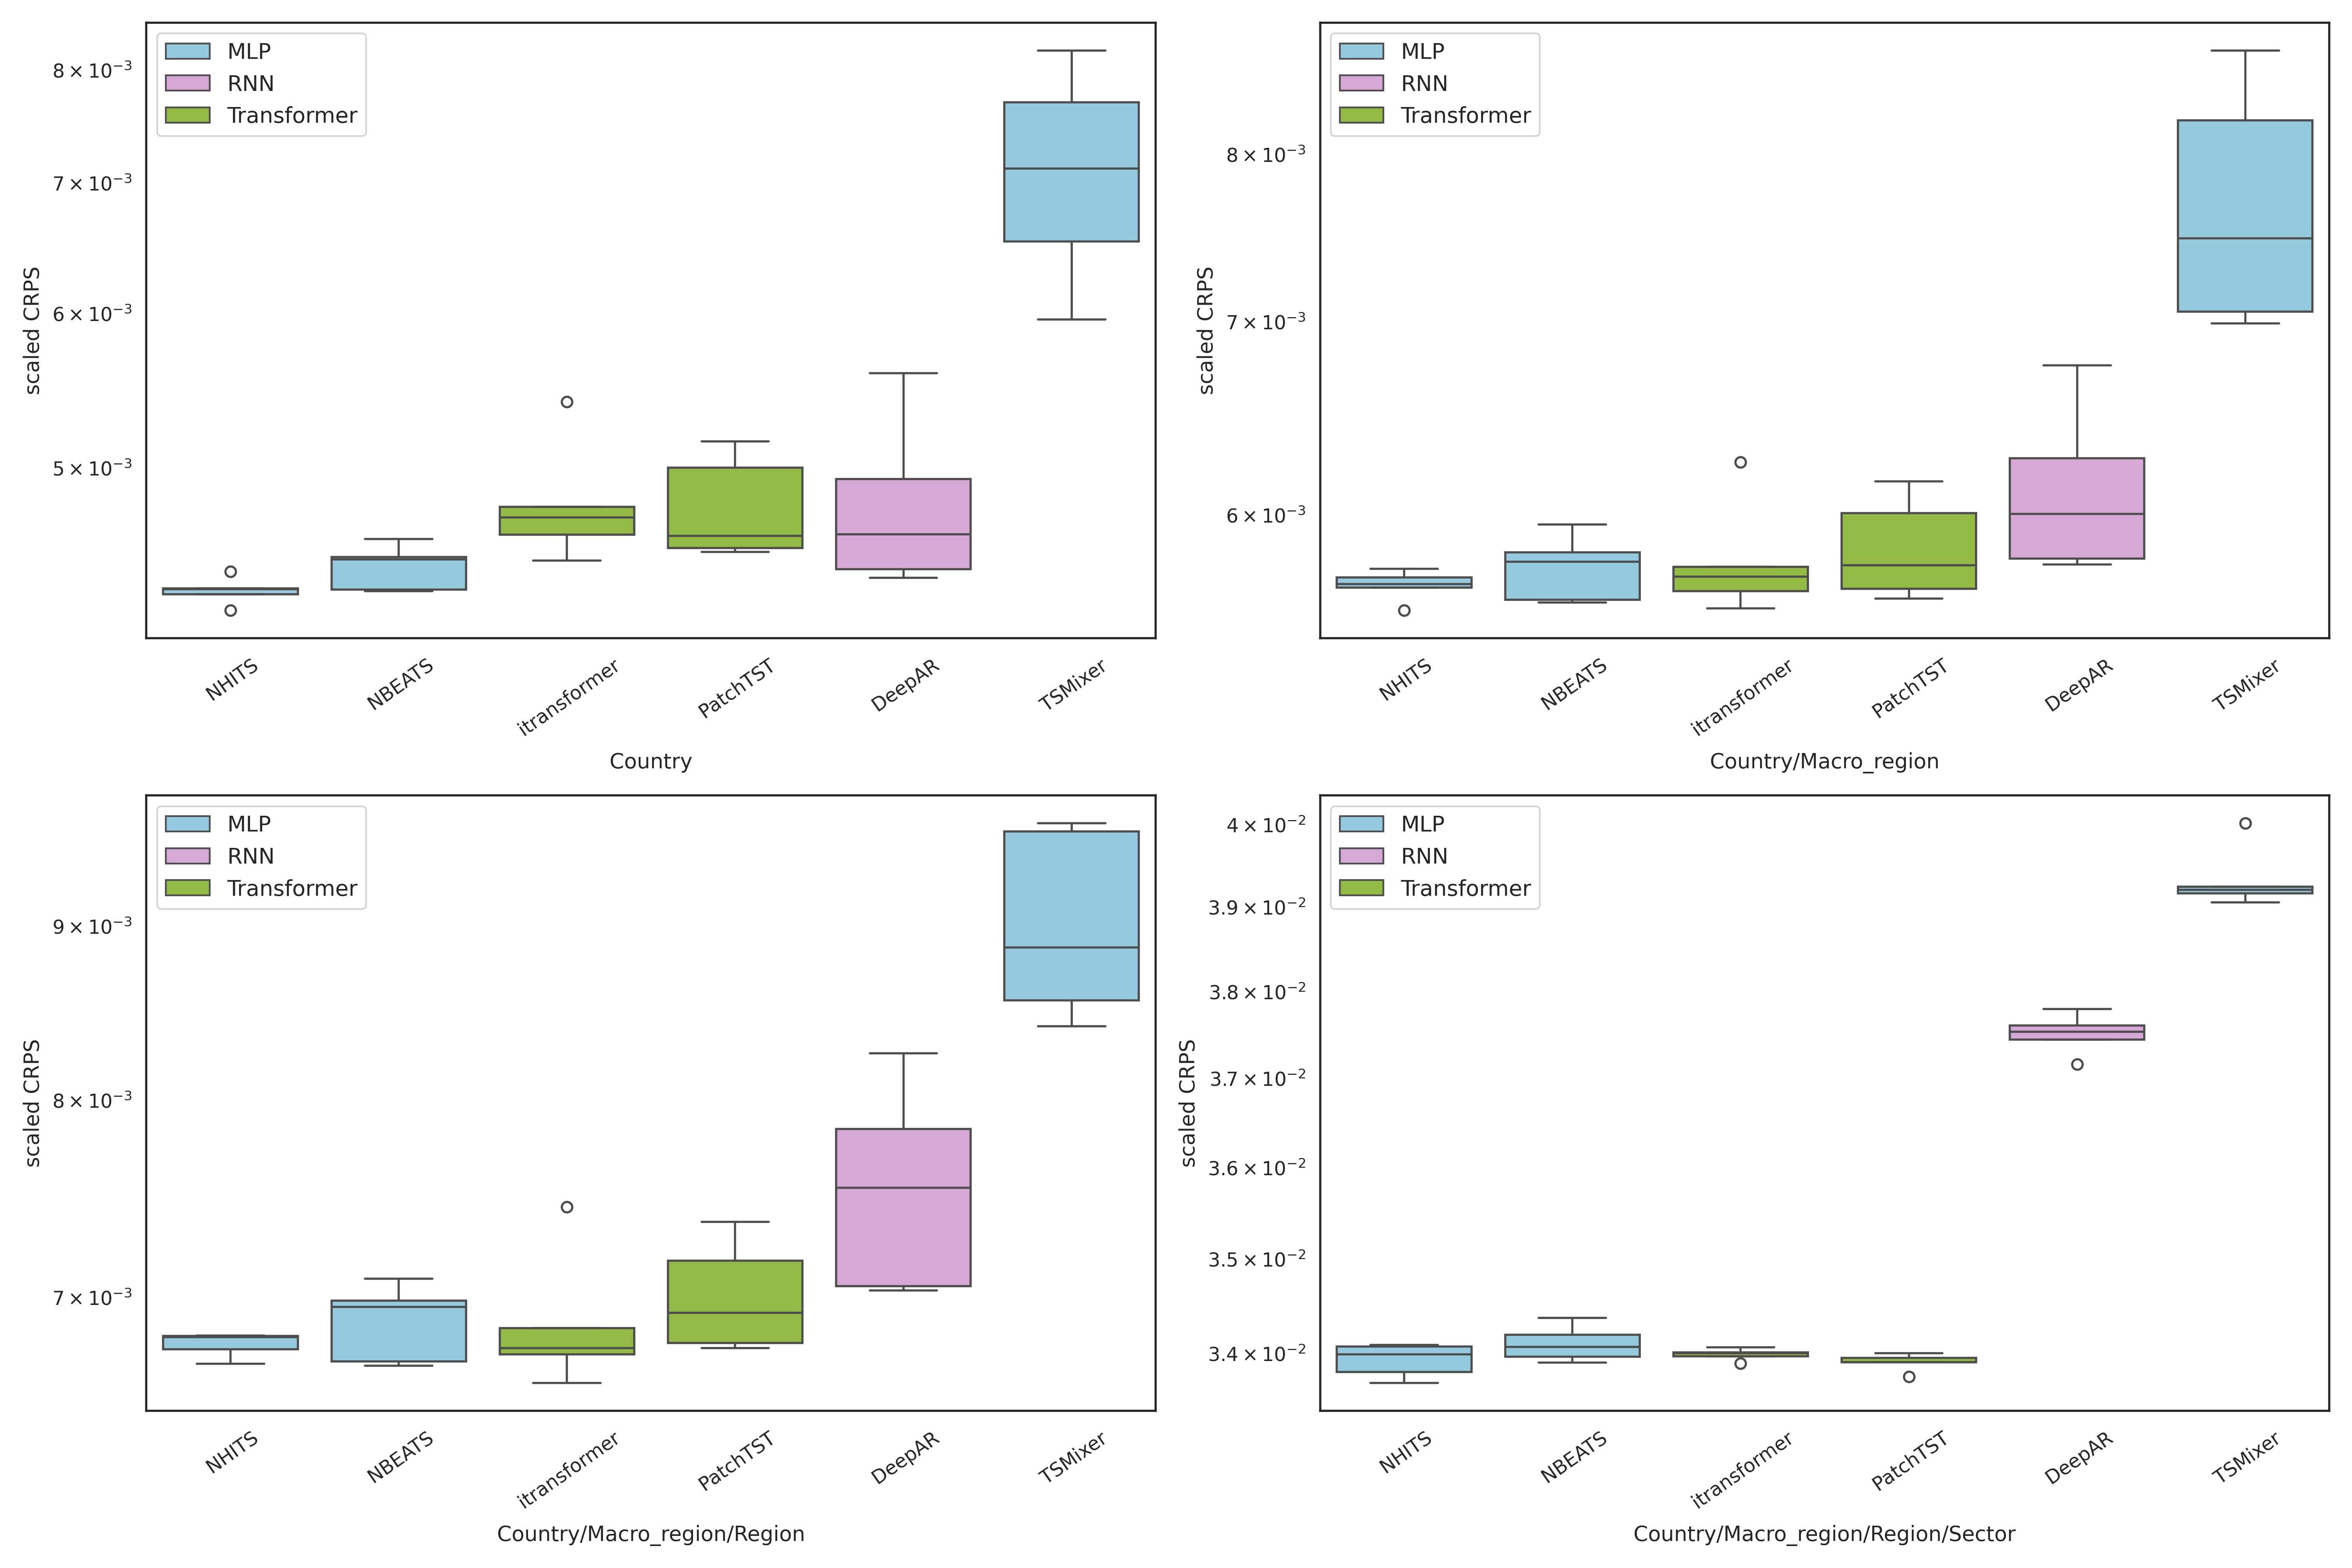
\includegraphics[width=\linewidth]{perf_HierE2E_models.png}
    \caption{Benchmark of model performances at each level of the hierarchy. Performance is measured as the average over 5 runs when the model is used as the main forecaster within the HierE2E framework. The benchmarked models include our choice of model (NBEATS, NHITS) and the original DeepAR model from the HierE2E paper. We also include three recent architecture including TSMixer and it}
    \label{fig:crps_model_comparison}
\end{figure}

\begin{figure}[h]
    \centering
    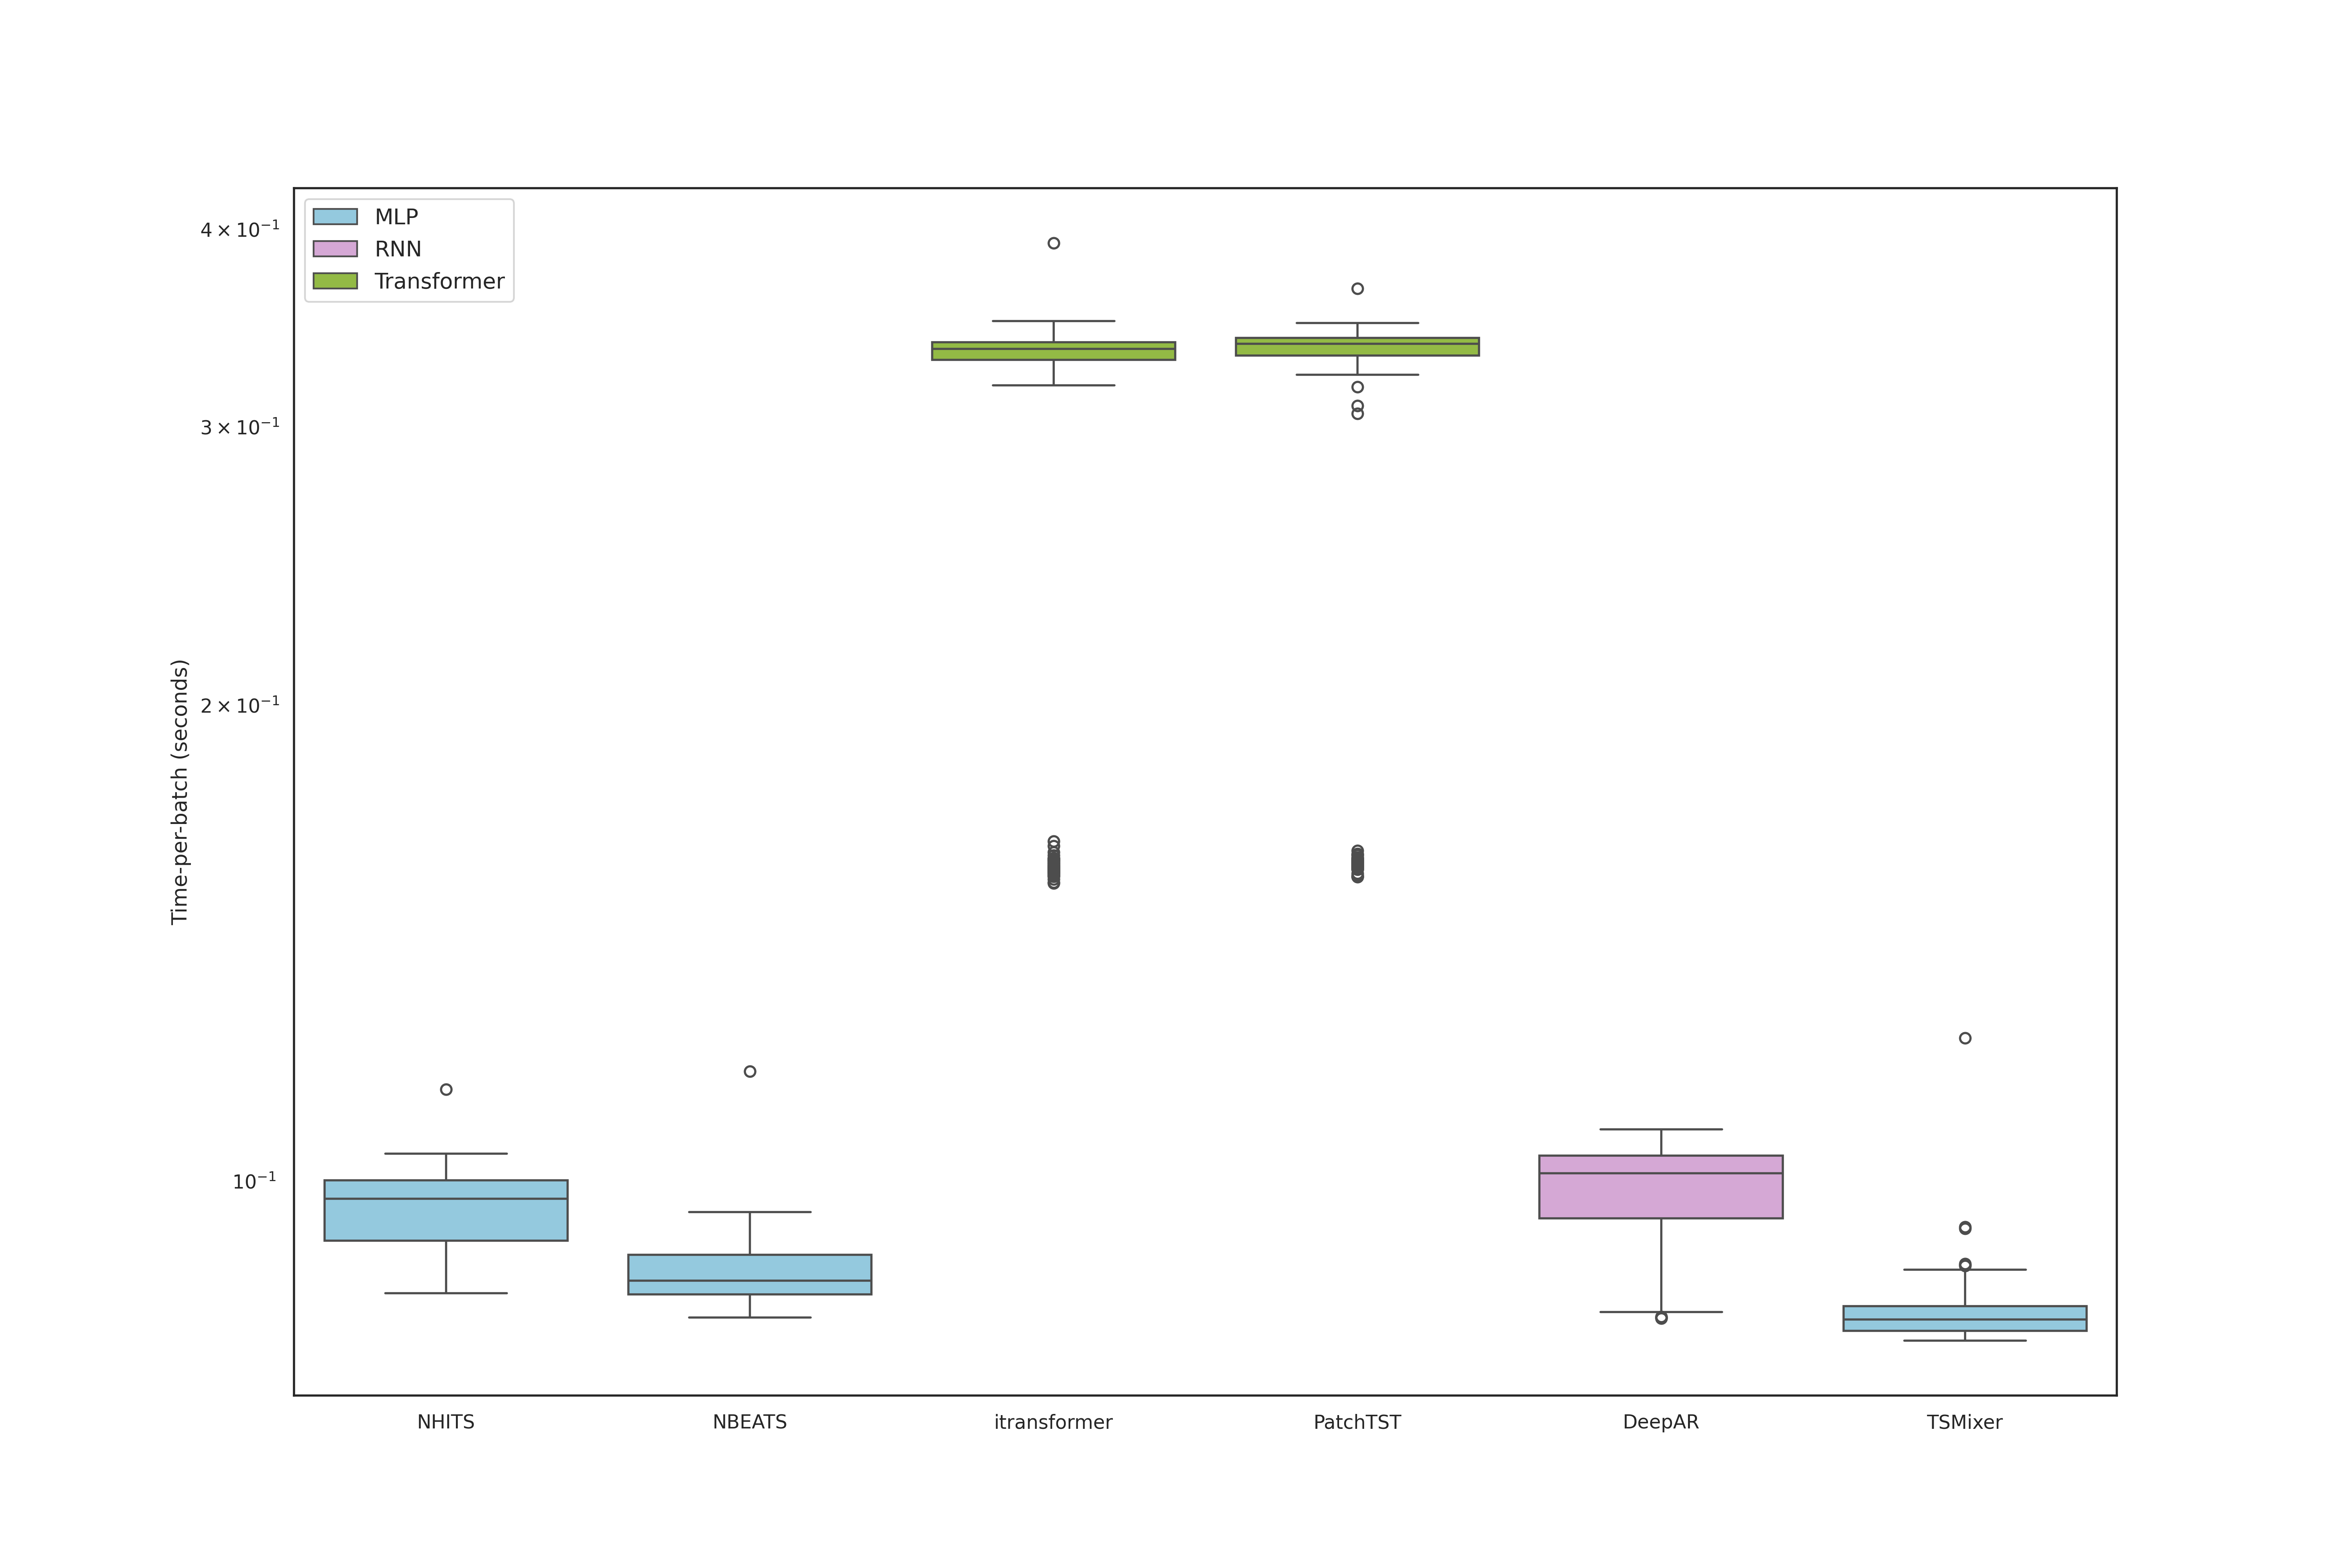
\includegraphics[width=\linewidth]{perf_time_HierE2E.png}
    \caption{Time per training batch for each forecasting architecture. Transformer-based models are significantly slower than MLP-based alternatives.}
    \label{fig:training_time_comparison}
\end{figure}


\end{document}